%  A simple AAU report template.
%  2015-05-08 v. 1.2.0
%  Copyright 2010-2015 by Jesper Kjær Nielsen <jkn@es.aau.dk>
%
%  This is free software: you can redistribute it and/or modify
%  it under the terms of the GNU General Public License as published by
%  the Free Software Foundation, either version 3 of the License, or
%  (at your option) any later version.
%
%  This is distributed in the hope that it will be useful,
%  but WITHOUT ANY WARRANTY; without even the implied warranty of
%  MERCHANTABILITY or FITNESS FOR A PARTICULAR PURPOSE.  See the
%  GNU General Public License for more details.
%
%  You can find the GNU General Public License at <http://www.gnu.org/licenses/>.
%
%  A simple AAU report template.
%  2015-05-08 v. 1.2.0
%  Copyright 2010-2015 by Jesper Kjær Nielsen <jkn@es.aau.dk>
%
%  This is free software: you can redistribute it and/or modify
%  it under the terms of the GNU General Public License as published by
%  the Free Software Foundation, either version 3 of the License, or
%  (at your option) any later version.
%
%  This is distributed in the hope that it will be useful,
%  but WITHOUT ANY WARRANTY; without even the implied warranty of
%  MERCHANTABILITY or FITNESS FOR A PARTICULAR PURPOSE.  See the
%  GNU General Public License for more details.
%
%  You can find the GNU General Public License at <http://www.gnu.org/licenses/>.
%
\documentclass[11pt,twoside,a4paper,openright]{report}
%%%%%%%%%%%%%%%%%%%%%%%%%%%%%%%%%%%%%%%%%%%%%%%%
% Language, Encoding and Fonts
% http://en.wikibooks.org/wiki/LaTeX/Internationalization
%%%%%%%%%%%%%%%%%%%%%%%%%%%%%%%%%%%%%%%%%%%%%%%%
% Select encoding of your inputs. Depends on
% your operating system and its default input
% encoding. Typically, you should use
%   Linux  : utf8 (most modern Linux distributions)
%            latin1 
%   Windows: ansinew
%            latin1 (works in most cases)
%   Mac    : applemac
% Notice that you can manually change the input
% encoding of your files by selecting "save as"
% an select the desired input encoding. 
\usepackage[utf8]{inputenc}
% Make latex understand and use the typographic
% rules of the language used in the document.
\usepackage[danish,english]{babel}
% Use the palatino font
\usepackage[sc]{mathpazo}
\linespread{1.05}         % Palatino needs more leading (space between lines)
% Choose the font encoding
\usepackage[T1]{fontenc}
%%%%%%%%%%%%%%%%%%%%%%%%%%%%%%%%%%%%%%%%%%%%%%%%
% Graphics and Tables
% http://en.wikibooks.org/wiki/LaTeX/Importing_Graphics
% http://en.wikibooks.org/wiki/LaTeX/Tables
% http://en.wikibooks.org/wiki/LaTeX/Colors
%%%%%%%%%%%%%%%%%%%%%%%%%%%%%%%%%%%%%%%%%%%%%%%%
% load a colour package
\usepackage{xcolor}
\definecolor{aaublue}{RGB}{33,26,82}% dark blue
% The standard graphics inclusion package
\usepackage{graphicx}
% Set up how figure and table captions are displayed
\usepackage{caption}
\captionsetup{%
  font=footnotesize,% set font size to footnotesize
  labelfont=bf % bold label (e.g., Figure 3.2) font
}
% Make the standard latex tables look so much better
\usepackage{array,booktabs}
% Enable the use of frames around, e.g., theorems
% The framed package is used in the example environment
\usepackage{framed}

%%%%%%%%%%%%%%%%%%%%%%%%%%%%%%%%%%%%%%%%%%%%%%%%
% Mathematics
% http://en.wikibooks.org/wiki/LaTeX/Mathematics
%%%%%%%%%%%%%%%%%%%%%%%%%%%%%%%%%%%%%%%%%%%%%%%%
% Defines new environments such as equation,
% align and split 
\usepackage{amsmath}
% Adds new math symbols
\usepackage{amssymb}
% Use theorems in your document
% The ntheorem package is also used for the example environment
% When using thmmarks, amsmath must be an option as well. Otherwise \eqref doesn't work anymore.
\usepackage[framed,amsmath,thmmarks]{ntheorem}

%%%%%%%%%%%%%%%%%%%%%%%%%%%%%%%%%%%%%%%%%%%%%%%%
% Page Layout
% http://en.wikibooks.org/wiki/LaTeX/Page_Layout
%%%%%%%%%%%%%%%%%%%%%%%%%%%%%%%%%%%%%%%%%%%%%%%%
% Change margins, papersize, etc of the document
\usepackage[
  inner=28mm,% left margin on an odd page
  outer=41mm,% right margin on an odd page
  ]{geometry}
% Modify how \chapter, \section, etc. look
% The titlesec package is very configureable
\usepackage{titlesec}
\titleformat{\chapter}[display]{\normalfont\huge\bfseries}{\chaptertitlename\ \thechapter}{20pt}{\Huge}
\titleformat*{\section}{\normalfont\Large\bfseries}
\titleformat*{\subsection}{\normalfont\large\bfseries}
\titleformat*{\subsubsection}{\normalfont\normalsize\bfseries}
%\titleformat*{\paragraph}{\normalfont\normalsize\bfseries}
%\titleformat*{\subparagraph}{\normalfont\normalsize\bfseries}

% Clear empty pages between chapters
\let\origdoublepage\cleardoublepage
\newcommand{\clearemptydoublepage}{%
  \clearpage
  {\pagestyle{empty}\origdoublepage}%
}
\let\cleardoublepage\clearemptydoublepage

% Change the headers and footers
\usepackage{fancyhdr}
\pagestyle{fancy}
\fancyhf{} %delete everything
\renewcommand{\headrulewidth}{0pt} %remove the horizontal line in the header
\fancyhead[RE]{\small\nouppercase\leftmark} %even page - chapter title
\fancyhead[LO]{\small\nouppercase\rightmark} %uneven page - section title
\fancyhead[LE,RO]{\thepage} %page number on all pages
% Do not stretch the content of a page. Instead,
% insert white space at the bottom of the page
\raggedbottom
% Enable arithmetics with length. Useful when
% typesetting the layout.
\usepackage{calc}

%%%%%%%%%%%%%%%%%%%%%%%%%%%%%%%%%%%%%%%%%%%%%%%%
% Bibliography
% http://en.wikibooks.org/wiki/LaTeX/Bibliography_Management
%%%%%%%%%%%%%%%%%%%%%%%%%%%%%%%%%%%%%%%%%%%%%%%%
\usepackage[backend=bibtex,
  bibencoding=utf8
  ]{biblatex}
\addbibresource{bib/mybib}

%%%%%%%%%%%%%%%%%%%%%%%%%%%%%%%%%%%%%%%%%%%%%%%%
% Misc
%%%%%%%%%%%%%%%%%%%%%%%%%%%%%%%%%%%%%%%%%%%%%%%%
% Add bibliography and index to the table of
% contents
\usepackage[nottoc]{tocbibind}
% Add the command \pageref{LastPage} which refers to the
% page number of the last page
\usepackage{lastpage}
% Add todo notes in the margin of the document
\usepackage[
%  disable, %turn off todonotes
  colorinlistoftodos, %enable a coloured square in the list of todos
  textwidth=\marginparwidth, %set the width of the todonotes
  textsize=scriptsize, %size of the text in the todonotes
  ]{todonotes}

%%%%%%%%%%%%%%%%%%%%%%%%%%%%%%%%%%%%%%%%%%%%%%%%
% Hyperlinks
% http://en.wikibooks.org/wiki/LaTeX/Hyperlinks
%%%%%%%%%%%%%%%%%%%%%%%%%%%%%%%%%%%%%%%%%%%%%%%%
% Enable hyperlinks and insert info into the pdf
% file. Hypperref should be loaded as one of the 
% last packages
\usepackage{hyperref}
\hypersetup{%
	pdfpagelabels=true,%
	plainpages=false,%
	pdfauthor={Author(s)},%
	pdftitle={Title},%
	pdfsubject={Subject},%
	bookmarksnumbered=true,%
	colorlinks=false,%
	citecolor=black,%
	filecolor=black,%
	linkcolor=black,% you should probably change this to black before printing
	urlcolor=black,%
	pdfstartview=FitH%
}
\usepackage{xcolor}
\usepackage{tcolorbox}% package inclusion and set up of the document
% see, e.g., http://en.wikibooks.org/wiki/LaTeX/Formatting#Hyphenation
% for more information on word hyphenation
\hyphenation{ex-am-ple hy-phen-a-tion short}
\hyphenation{long la-tex}% 
%  A simple AAU report template.
%  2015-05-08 v. 1.2.0
%  Copyright 2010-2015 by Jesper Kjær Nielsen <jkn@es.aau.dk>
%
%  This is free software: you can redistribute it and/or modify
%  it under the terms of the GNU General Public License as published by
%  the Free Software Foundation, either version 3 of the License, or
%  (at your option) any later version.
%
%  This is distributed in the hope that it will be useful,
%  but WITHOUT ANY WARRANTY; without even the implied warranty of
%  MERCHANTABILITY or FITNESS FOR A PARTICULAR PURPOSE.  See the
%  GNU General Public License for more details.
%
%  You can find the GNU General Public License at <http://www.gnu.org/licenses/>.
%
%
%
% see, e.g., http://en.wikibooks.org/wiki/LaTeX/Customizing_LaTeX#New_commands
% for more information on how to create macros

%%%%%%%%%%%%%%%%%%%%%%%%%%%%%%%%%%%%%%%%%%%%%%%%
% Macros for the titlepage
%%%%%%%%%%%%%%%%%%%%%%%%%%%%%%%%%%%%%%%%%%%%%%%%
%Creates the aau titlepage
\newcommand{\aautitlepage}[3]{%
  {
    %set up various length
    \ifx\titlepageleftcolumnwidth\undefined
      \newlength{\titlepageleftcolumnwidth}
      \newlength{\titlepagerightcolumnwidth}
    \fi
    \setlength{\titlepageleftcolumnwidth}{0.5\textwidth-\tabcolsep}
    \setlength{\titlepagerightcolumnwidth}{\textwidth-2\tabcolsep-\titlepageleftcolumnwidth}
    %create title page
    \thispagestyle{empty}
    \noindent%
    \begin{tabular}{@{}ll@{}}
      \parbox{\titlepageleftcolumnwidth}{
        \iflanguage{danish}{%
          \includegraphics[width=\titlepageleftcolumnwidth]{figures/aau_logo_da}
        }{%
          \includegraphics[width=\titlepageleftcolumnwidth]{figures/aau_logo_en}
        }
      } &
      \parbox{\titlepagerightcolumnwidth}{\raggedleft\sf\small
        #2
      }\bigskip\\
       #1 &
      \parbox[t]{\titlepagerightcolumnwidth}{%
      \textbf{Abstract:}\bigskip\par
        \fbox{\parbox{\titlepagerightcolumnwidth-2\fboxsep-2\fboxrule}{%
          #3
        }}
      }\\
    \end{tabular}
    \vfill
    \iflanguage{danish}{%
      \noindent{\footnotesize\emph{Rapportens indhold er frit tilgængeligt, men offentliggørelse (med kildeangivelse) må kun ske efter aftale med forfatterne.}}
    }{%
      \noindent{\footnotesize\emph{The content of this report is freely available, but publication (with reference) may only be pursued due to agreement with the author.}}
    }
    \clearpage
  }
}

%Create english project info
\newcommand{\englishprojectinfo}[8]{%
  \parbox[t]{\titlepageleftcolumnwidth}{
    \textbf{Title:}\\ #1\bigskip\par
    \textbf{Theme:}\\ #2\bigskip\par
    \textbf{Project Period:}\\ #3\bigskip\par
    \textbf{Project Group:}\\ #4\bigskip\par
    \textbf{Participant(s):}\\ #5\bigskip\par
    \textbf{Supervisor(s):}\\ #6\bigskip\par
    \textbf{Copies:} #7\bigskip\par
    \textbf{Page Numbers:} \pageref{LastPage}\bigskip\par
    \textbf{Date of Completion:}\\ #8
  }
}

%Create danish project info
\newcommand{\danishprojectinfo}[8]{%
  \parbox[t]{\titlepageleftcolumnwidth}{
    \textbf{Titel:}\\ #1\bigskip\par
    \textbf{Tema:}\\ #2\bigskip\par
    \textbf{Projektperiode:}\\ #3\bigskip\par
    \textbf{Projektgruppe:}\\ #4\bigskip\par
    \textbf{Deltager(e):}\\ #5\bigskip\par
    \textbf{Vejleder(e):}\\ #6\bigskip\par
    \textbf{Oplagstal:} #7\bigskip\par
    \textbf{Sidetal:} \pageref{LastPage}\bigskip\par
    \textbf{Afleveringsdato:}\\ #8
  }
}

%%%%%%%%%%%%%%%%%%%%%%%%%%%%%%%%%%%%%%%%%%%%%%%%
% An example environment
%%%%%%%%%%%%%%%%%%%%%%%%%%%%%%%%%%%%%%%%%%%%%%%%
\theoremheaderfont{\normalfont\bfseries}
\theorembodyfont{\normalfont}
\theoremstyle{break}
\def\theoremframecommand{{\color{gray!50}\vrule width 5pt \hspace{5pt}}}
\newshadedtheorem{exa}{Example}[chapter]
\newenvironment{example}[1]{%
		\begin{exa}[#1]
}{%
		\end{exa}
}
\usepackage{subfigure}% my new macros

% TIMELINE
% Milestone 1:  30.03 11.30 UTC (TOC)
% Milestone 2:  30.04./02.05 (First Draft)
% Milestone 3:  31.05 /01.06 (Review and finalization of work)
% Milestone 4:  14.06 (sending draft for Review to IEA Wind Community)
% Milestone 5:  31.07 - 15.08 (implementing feedback and final review)
% Milestone 6:  20.08.2019 Submission to IEA Task 11 OA  and IEA Wind secretary
% Milestone 7:  xx.10.2021 Acceptance for Publication by Task11 with minor changes
% Milestone 8:  31.12.2021 Submission of final version at IEA and OAbook

%%%%%%%%%%%%%%%%%%%%%%%%%%%%%%%%%%%%%%%%%%%%%%%%%%%%%%%%%%
%%%% FINAL CORRECTED VERSION                       %%%%%%%
%%%%%%%%%%%%%%%%%%%%%%%%%%%%%%%%%%%%%%%%%%%%%%%%%%%%%%%%%%

\begin{document}
\noindent

%frontmatter
\pagestyle{empty} %disable headers and footers
\pagenumbering{roman} %use roman page numbering in the frontmatter
%  A simple AAU report template.
%  2015-05-08 v. 1.2.0
%  Copyright 2010-2015 by Jesper Kjær Nielsen <jkn@es.aau.dk>
%
%  This is free software: you can redistribute it and/or modify
%  it under the terms of the GNU General Public License as published by
%  the Free Software Foundation, either version 3 of the License, or
%  (at your option) any later version.
%
%  This is distributed in the hope that it will be useful,
%  but WITHOUT ANY WARRANTY; without even the implied warranty of
%  MERCHANTABILITY or FITNESS FOR A PARTICULAR PURPOSE.  See the
%  GNU General Public License for more details.
%
%  You can find the GNU General Public License at <http://www.gnu.org/licenses/>.
%
\pdfbookmark[0]{Front page}{label:frontpage}%
\begin{titlepage}
  \addtolength{\hoffset}{0.5\evensidemargin-0.5\oddsidemargin} %set equal margins on the frontpage - remove this line if you want default margins
  \noindent%
  \begin{tabular}{@{}p{\textwidth}@{}}
    \toprule[2pt]
    \midrule
    \vspace{0.2cm}
    \begin{center}
    \Huge{\textbf{
%      EXPERT GROUP REPORT ON
RECOMMENDED PRACTICES FOR THE IMPLEMENTATION OF
 RENEWABLE ENERGY FORECASTING SOLUTIONS% insert your title here
    }}
    \end{center}
    \begin{center}
      \Large{
        - Part 4:  Meteorological and Power Data Requirements for real-time forecasting Applications-% insert your subtitle here
      }
    \end{center}
    \vspace{0.2cm}\\
    \midrule
    \toprule[2pt]
  \end{tabular}
  \vspace{4 cm}
  \begin{center}
    {\large
      \color{blue}{1. DRAFT EDITION 2021} \\ 
      %\color{green} POST PUBLIC REVIEW VERSION \\ \color{black}%Insert document type (e.g., Project Report)
    }
    \vspace{0.2cm}
    {\Large
      Draft for Review by Stakeholders prior to submission to the Executive Committee of the International Energy Agency Implementing Agreement in September 2021%Insert your group name or real names here
      \\
    %  {\color{blue}{Comment from SW (25.06.2021: Title of the series “wind power forecasting” does not fit to solar energy-> Can we publish the report outside the series or with a different title? Other solutions?}}
    }
  \end{center}
  \vfill
  \begin{center}
  Prepared in 2021 as part of the IEA Wind Task 36, WP 3.3.
  \end{center}
\end{titlepage}
\clearpage
\thispagestyle{empty}
{\small
\strut\vfill % push the content to the bottom of the page
\noindent Copyright \copyright{} IEA Wind Task 36\par
\vspace{0.2cm}
\noindent Edited by: Corinna Möhrlen, ???\\
Document Version: 1.0\\
\today
}
\clearpage
\cleardoublepage
\pdfbookmark[0]{Contents}{label:contents}
\pagestyle{fancy} %enable headers and footers again
\tableofcontents
%%%% REMEMBER TO REMOVE BEFORE PUBLICATION %%%%%%%
%\listoftodos
%%%%%%%%%%%%%%%%%%%%%%%%%%%%%%%%%%%%%%%%%%%%%%%%%%%
\chapter*{Preface\markboth{Preface}{Preface}}\label{ch:preface}
\addcontentsline{toc}{chapter}{Preface}
This recommended practice document is the result of a collaborative work that has been edited by the undersigning authors in alignment with many discussions at project meetings, workshops and personal communication with colleagues, stakeholders and other interested persons throughout the phase 1 of the IEA Wind Task 36 (2019-2021) as part of workpackage 3.3. 

The editors want to thank everybody that has been part of the meetings, workshops and sessions and contributed in the discussions, provided feedback or other input throughout the past 3 years. 


\vspace{\baselineskip}\hfill IEA Wind Task 36, \today \\ \\ \\
\textbf{Editors:} \\ 
Dr. Corinna M\"ohrlen (WEPROG) {\footnotesize <com@weprog.com>}\\
Author 2 () {\footnotesize <>}\\
Author 3 () {\footnotesize <>}\\
Author 4 () {\footnotesize <>}\\




\iffalse
\vfill\noindent
\begin{minipage}[b]{0.45\textwidth}
 \centering
 %\rule{\textwidth}{0.5pt}\\
  Dr. Corinna M\"ohrlen \\ {\footnotesize <com@weprog.com>}
\end{minipage}
\hfill
\begin{minipage}[b]{0.45\textwidth}
 \centering
 %\rule{\textwidth}{0.5pt}\\
  Dr. John Zack (UL AWS Truepower)\\  {\footnotesize <john.zack@awstruepower.com>}
\end{minipage}
\vspace{3\baselineskip}
\begin{center}
\begin{minipage}[b]{0.45\textwidth}
 \centering
 %\rule{\textwidth}{0.5pt}
  Dr. Jakob W. Messner (Anemos Analytics)\\ {\footnotesize <jakob.messner@posteo.net>}
 \end{minipage}
 \hfill
\begin{minipage}[b]{0.45\textwidth}
 \centering
 %\rule{\textwidth}{0.5pt}\\
  Dr. Jethro Browell (University of Strathclyde)\\  {\footnotesize <jethro.browell@strath.ac.uk>}
 \end{minipage}
\end{center}
\fi
{\color{blue}{
\textbf{WORKING COMMENTS}\\

Please put your abbreviation to the headlines where you find a
{\color{magenta}{Contributing author: }}

Where you suggest to add a section, PLEASE add the text {\color{magenta}{Contributing author: }} to the section heading\\


Abbreviations:\\
AK: Anton Kaifel \\
CK: Carmen K{\"o}hler\\
COM: Corinna M{\"o}hrlen\\
ES: Elliot Simon\\
GG: Gregor Giebel\\
IW: Ines W{\"u}rth\\
IP: Isabel Peinke \\
JY: Jie Yan\\
JB: Jethro Browell\\
JR: Jan Remund \\
JZ: John Zack\\
RP: Rui Pestana\\
SW: Styefan Wilbert \\
}}

\cleardoublepage
%mainmatter
\pagenumbering{arabic} %use arabic page numbering in the mainmatter

\chapter{Background and Objectives } \label{ch:introduction}
%%\color{green} POST PUBLIC REVIEW VERSION \\ \color{black}

\noindent
\begin{comment}
\begin{tcolorbox}
\parbox{\textwidth}{
\emph{\textbf{Key Points}\\
This is the fourth part of a series of four recommended practice documents that deals with the development and operation of renewable energy forecasting solutions for the power market.
This part provides information and guidelines for the best practices of met measurements in the real-time operation of grid operators....
}}
\end{tcolorbox}
\end{comment}
{\color{red}{\textbf{Who is our target user and how do we address this user \\
authority ? end-user ? ...?}}}

\section{BEFORE YOU START READING}

This is the forth part of a series of four recommended practice documents that deal with the development and operation of forecasting solutions in the power market. 
The first part  “Forecast Solution Selection Process” deals with the selection and background information necessary to collect and evaluate when developing or renewing a forecasting solution for the power market. 
The second part “Design and Execution of Benchmarks and Trials”, of the series deal with benchmarks and trials in order to test or evaluate different forecasting solutions against each other and the fit-for-purpose. 
The third part “Forecast Solution Evaluation”, which is the current document, provides information and guidelines regarding effective evaluation of forecasts, forecast solutions and benchmarks and trials.


\section{Introduction {\color{magenta}{Contributing author: COM}}}

Meteorological measurements provide an independent measure of the wind and solar resource and weather situation at any given time. This information can and is, as technology enhances, not only an obligation that stems from technical requirements of the system operator, but is also used to optimise the operation of renewable power plants and electricity grids.
For both the system operator and the power plant operator, these measurements are an independent signal at the power plant that can warn about critical weather and provide an indication on whether the power plants work at their expected performance level. For the transmission system operator, such measurements can additionally be used for situational awareness of the weather in the control area that may affect the transmission lines. They also provide a second means of verification, whether the power signal at a given power plant is malfunctioning in situations that may be critical in terms of grid operation.

Data assimilation with independent measurements from power plants have also been tested by meteorological centres (e.g. \cite{Marquis2012,EWELINE2011}). One of the most important findings so far is that the quality of data provided is the most essential issue to be solved in order to gain higher quality forecasts with such measurements. In other words, if there is no specific effort put into standardisation of requirements in the power industry, the benefits can not be achieved.

This recommended practice (RP) is aimed to provide background information on meteorological instrumentation, their recommended setup, maintenance, quality control and use in the real-time environment of wind and solar power generation plants. Information on use of real-time power and other operational data in forecasting systems is also included.  The document provides practical guidelines for quality control and recommended standards to be applied in the setup and calibration of instrumentation  when entering the operational phase of wind and solar projects and for applications  relevant to plant operators, system operators, power traders or balance responsible parties. 

%comment COM 28.06.2021: the below comments have been implemented today in the above paragraph, which may still need adjustment along the way.... 
%{\color{blue}{Comment from SW (25.06.2021: Do we really also address “setup […] phase”?}}
%{\color{green}{Commend COM (2021-06-27): It would be good to have the setup also discussed in a rudimentary way, i.e. are there differences in the conditions to what is covered by the available standards ? If we can refer to a standard as the recommended way of setting up instrumentation, that would be ideal. In both wind and solar, I'd assume that there is not much difference, where to setup the instruments on a e.g. met mast or within the power plant to retrieve undistrubed data...}}

{\color{green}{Commend COM (2021-06-30): We need to incorporate the power measurements here also --- this is an outstanding task! }}

\section{Use and Application of real-time Meteorological Measurements }
{\color{magenta}{Contributing author: JY, JZ, COM}}

In this section, we will define and discuss the use of meteorological measurements for real-time application and especially make the distinction to non-real-time use and applications such as resource assessment. 


\subsection{Real-time applications vs. non-real time applications}
% {\color{blue}{Comment from SW (25.06.2021: I think  “resource assessment” in the title was too general. This is also an issue in table 1.1 and other parts of the text. It could be understood  including all uses and time resolutions or as only referring to the assessments before the plant construction. Also plant control required real time operation. }}
%This section discusses the differences between deploying and operating measurement systems for these two types of applications.
The main difference between meteorological measurements used for non-real time applications such as resource assessments or periodic power plant monitoring and real-time applications such as forecasting, plant control and situational awareness is: 
\begin{enumerate}
    \item \textbf{Non-real time applications}\\
    here the aim is to collect enough data in all known weather regimes to make a reliable prediction of the life-time yield of a power plant at a specific location or to allow the evaluation of its performance for time intervals such as days, months or years. Gaps and missing data are not as critical in the time series as long as the overall goal is achieved. Temporarily erroneous data reduces the overall quality of the result, but might not cause important errors, as long as most of the data are ok or as long as errors cancel out.
    \item \textbf{Real-time Applications}\\
    here the aim is to have reliable information about the current weather situation; gaps (missing data) are more critical as for these times, forecasts or plant control parameters cannot be generated or adapted with the help of measurements. Forecasts and other control options with lower quality must then be used. Temporarily erroneous data is more critical as the forecasts or plant control might lead to energetic and economic inefficiencies, system security issues etc.
\end{enumerate}

Therefore, the instrumentation and requirements for the signal quality is slightly different and needs to be taken into consideration. The following table defines the main differences:

\begin{table}[h!]
\begin{center}
 \begin{tabular}{|| l l l ||}
 \hline\hline
  & & \\ 
\textbf{Use} & \textbf{Non real-time Application} & \textbf{Real-time Application} \\ 
 \hline \hline
& \textbf{Wind Power related} & \\\hline \hline
Yield & long-term trends & current weather \\
Wake effects & no issue & important consideration \\
... & & \\ \hline \hline
& \textbf{Solar Power related} & \\ \hline \hline
Shading & average over life-time & current clouds/obstacles\\ 
Performance Loss Rates & module degradation & unavailability \\
Transposition GHI -> GTI & climate dependent & calculation method \\
... & & \\ \hline \hline
& \textbf{General}  & \\ \hline \hline
BIAS & near-zero required & not as critical \\
Extreme events & enlarge data collection & critical \\
Plant availability & n/a & important for forecasting \\
Uncertainty & Calculation method & current weather related \\
Temperature & average, min, max & current temperature\\
... & & \\ \hline \hline
\end{tabular}
\caption{\textit{Differences between use of meteorological measurements for resource assessment and real-time applications}}
\label{tab:qlimit}
\end{center}
\end{table}

% {\color{blue}{Comment from SW (25.06.2021: the table should be discussed. E.g.:\\
%Non real time is not only  for long term data series.\\
%Shading must be known as time series, too\\
%Loss rates for real time applications “unavailability” is most likely not enough }}

%{\color{blue}{ ... Johns comments are implemented and outcommented below - but maybe we find even more to add ...? }}

\iffalse
{\color{blue}{I am not clear  on the significance/value to the user of some of the items in Table 1.1
I was thinking that it would be more valuable to summarize the relative importance of
specific measurement attributes.  Here are my initial thoughts:
Measurement Attribute: Bias\\
----------------------------\\
Resource Assessment - near-zero bias in the measurement is critical since a small bias
over a long period can significantly impact of the estimated energy yield of a  facility

Forecasting:  Modest biases in measurements are not nearly as critical; ability to measure changes
over short time periods is more essential

Measurement Attribute: Measurement in Extreme Weather Conditions\\
-----------------------------------------------------------------\\
Resource Assessment: lost data during infrequent extreme weather conditions (e.g. high winds, icing etc.)
is not critical because these represent a very small amount of the total energy production (in fact under
such conditions there often may be no energy produced)

Forecasting: Ability to measure data in extreme conditions is very important because the foreacsting
of extreme weather shutdowns is critical for many operational purposes

Measurement Attribute: Impact of Wakes\\
---------------------------------------
Resource Assessment:  measurements are typically made before project development so turbine wakes are not an issue

Forecasting:  consideration of where the measurement is made relative to turbine locations is important
since the wind measurement may be impacted by wakes for some wind direcrtions


Measurement Attribute: Near Real-time availability of data\\
----------------------------------------------------------\\
Resource Assessment:  data does not typically need to be available in near real-time

Forecasting:  near real-time availability is often critical for use in forecasting applications
}}
\fi


\subsection{System Operation}

The key applications in system operation, where real-time meteorological measurements are required are: 

\begin{itemize}
    \item \textbf{Situational awareness in critical weather events}\\
    Critical weather events can cause severe security risks in grid operation. Forecasting and measurements assist to a large extend to make such events predictable and provide the necessary information to be able to act in advance. Such situational awareness is an important planning tool in grid operation, where penetration levels are above ca. 30\% of energy consumption.  Especially for wind generating power extreme winds can only be predicted by meteorological signals, due to the flattening of wind power curves in the wind ranges > ~12m/s. In this range, the power signal provides no local information to the system operator or the wind farm operator/balance responsible. 

    \item \textbf{High-Speed Shutdown events}\\
    During storm events, the critical parameter for the grid operation is the proportion of wind farms that are expected to enter into high-speed shutdown (HSSD) in any high penetration area. The risk and increased uncertainty for HSSD during storm events can result in the System Operator having to limit the wind generation in advance so that sufficient reserve is available.

    \item \textbf{Grid related down-regulation or curtailments}\\
    Grid related down-regulations or curtailments can be due to extreme weather events or technical problems at the electrical lines or controllers. Wind or solar radiation measurements can provide an independent signal to the system operator on the available active power potential, where this is not broadcasted and also provide the possibility to compute the lost power production due to the down/regulation. 
\end{itemize}


\subsection{Power plant operation {\color{blue}{Contributing author: IW/AC ?}}}

\subsubsection{Wind plant operation}
The key applications for wind plant operation, where real-time meteorological measurements are required are: 

\begin{itemize}
    \item \textbf{Wind turbine control}\\
    Due to wake effects on nacelle anemometer, independent site data from a met mast or LIDAR can assist the turbine controller to work more safe and efficient. 
    \item \textbf{Condition Monitoring}\\
    
    \item \textbf{Performance Evaluation and Optimisation}\\
    AI for performance monitoring (AK, maybe with support form Enercon?) 
    
\end{itemize}

\cite{Jing2020}

\subsubsection{Solar/PV plant operation}

The key applications for solar plant operation, where real-time meteorological measurements are required are: 

\begin{itemize}
    \item improving yield forecasting for the next minutes, hours and days for
        \begin{itemize}
            \item ramp rate control in PV power plants
            \item dispatch optimisation of power plans with storage
            \item optimisation of power plant operation for thermal plants (e.g. start up decisions)
        \end{itemize}
    \item power plant control
        \begin{itemize}
            \item optimisation of tracking of tracked PV or concentrating collectors
                \begin{itemize}
                    \item stow position for high wind speeds/gusts
                    \item optimal tracking angle for non concentrating tracked PV according to sky radiance distribution and shading
                    \item de-focusing of concentrating collectors at high DNIs
                \end{itemize}
            \item mass flow control in thermal collectors
            \item aim point control for solar tower plants
        \end{itemize}
\end{itemize}

Most of the real-time meteorological measurements are only required for large scale power plants. For tracking collectors of any size wind speed and direction measurements are required to allow for securing the collectors in the stow positions at high wind speeds. Depending on the solar thermal technology also further meteorological measurements may be required even for small systems. 

In the handbook \cite{nrelhandbook2017} and \cite{nrelhandbook2021}, it is noted that measurements of irradiance are complex therefore more expensive as general meteorological instruments, especially for measuring direct normal irradiance (DNI). The applications named in \cite{nrelhandbook2017} and \cite{nrelhandbook2021} developers utilise for irradiance data are:

\begin{itemize}
    \item Site resource analysis
     \item System design
     \item Plant operation 
     \item Developing, improving and testing models that use remote satellite sensing techniques or available surface meteorological observations
    \item Developing, improving and testing solar resource forecasting techniques.
\end{itemize}

The handbook \citep{nrelhandbook2021} also mentions a priority regarding the selection process of instrumentation:
\begin{enumerate}
    \item \textbf{Accuracy requirements}:\\
    Accuracy requirements need to be defined for the application/project and aligned with the associated levels of effort necessary to operate and maintain the measurement system on under these constraints. An overall cost-performance determination should be carried out to adapt the budget to the accuracy requirements and vice versa.
    \item \textbf{Reliability requirements}:\\
     Reliability can be achieved with redundant instrumentation and/or high quality instrumentation. Redundancy enhances and ensures confidence in data quality. Selection of multiple instruments need to be aligned with the accuracy needs. 
\end{enumerate}




\subsection{Power trading in electricity markets }
{\color{magenta}{Contributing author: COM, JB}}

The key applications for power trading and balancing, where real-time meteorological measurements are required are: 

\begin{itemize}
    \item \textbf{Short-term Forecasting using measurements}
    \item \textbf{Intra-day Power plant balancing}
    \item \textbf{Situational Awareness}
    \item \textbf{Refund calculation in curtailment situations}
\end{itemize}





\section{Available applicable Standards }
{\color{magenta}{Contributing author: COM}}{\color{blue}{ -- needs more attention}}

\subsection{Standards and Guidelines for Wind Measurements}\label{subsec:wind_standards}

For resource or site assessment in the planning phase of a wind farm an IEC standard exists [IEC, 2005] with an updated version 2 (IEC 61400-12-2:2013), that specifies which tests and what kind of criteria the instrumentation has to fulfil when used for the required tests to be carried out. The IEC 61400-12-2:2013 rules contain the following items:
\begin{itemize}
    \vspace{-0.2cm}\item Extreme winds
    \vspace{-0.4cm}\item Shear of vertical wind profile
    \vspace{-0.4cm}\item Flow inclination
    \vspace{-0.4cm}\item Background turbulence
    \vspace{-0.4cm}\item Wake turbulence
    \vspace{-0.4cm}\item Wind-speed distribution
\end{itemize}

The results of these tests have to be within a pre-defined range to be acceptable. In Appendix F of the 61400-12-1:2005 "Cup anemometer calibration procedure" the calibration of the instruments for measuring wind are specified.

The use of remote sensing for wind measurement was introduced in a new version 61400-12-1:2017. In Annex L guidelines for the classifications of remote sensing devices, for the verification of the performance and for the evaluation of uncertainties of the measurements are given. \\

MEASNET (MEASuring NETwork), the "international network for harmonised and recognized measurements in wind energy" has defined so called "Round Robin rules" for calibration of cup anemometers for wind energy [MEASNET, 2009], which are widely used. MEASNET has also under the EU project ACCUWIND published a number of guidelines regarding instrument calibration and measurement campaigns for the wind industry (Dahlberg et al., 2006, Pedersen et al. 2006, Eecen, 2006]. Lee [2008] found a way of calibrating wind direction sensors with an optical camera.

In 2016 MEASNET published Version 2.0 of a “Procedure for the evaluation of site-specific wind conditions” \cite{MEASNET2016}. This document gives guidance on measuring wind characteristics, and comprises  an  annex on wind measurement using remote sensing devices. It also includes guidance on how to set up measurement campaigns depending on the data required.

IEA Wind Task 32 and Task 11 published recommended practices RP-15 for ground-based remote sensing for wind resource assessment in 2013 \cite{RP15}. It covers different aspects of using lidars and sodars. An updated review version of 2020 \cite{clifton_review_2020} identifies recommendations from the relevant normative documents (RP-15, MEASNET 2016, IEC 61400-12-1:2017 Annex L) concerning characterisation, installation, operation, data analysis and verification of wind lidar .

The Annex D in IEC 61400-12-1:2005 standard states that the "implicit assumption of the method of this standard is that the 10 min mean power yield from a wind turbine is fully explained by the simultaneous 10 min mean wind speed measured at hub height, and the air density" [IEC, 2005, Annex D, Table D.1] and describes the associated measurement uncertainty evaluation principles.  In this respect, the standard refers to the "ISO Guide to the expression of Uncertainty in Measurements" \cite{jcgm2008,jcgm2009}, and its 2 supplements \cite{jcgm2008a,jcgm2011} from the Joint Committee for Guides in Meteorology (JCGM), where there are two types of measurement uncertainty that are to be accounted for in any standardised measurement taking: 
\begin{enumerate}
    \vspace{-0.2cm}\item systematic errors, often associated with offsets/bias of the measured quantity
    \vspace{-0.4cm}\item random errors, which are associated with the fact that 2 measurements of the same quantity are seldom the same
\end{enumerate}

In section 3.1.2 of the guide, [\cite{jcgm2008a,jcgm2011} it is stated that "the result of a measurement .. is only an approximation or estimate .. of the value of the measurand and thus is complete only when accompanied by a statement of the uncertainty ... of that estimate". Considering this definition, all measurements should ideally have an uncertainty term associated with it. This is impractical in real-time operations, where the value of the measurements lies in the availability of the data at a given time. Therefore, it is unrealistic to request uncertainty measures. However, it could be a standing data value that is determined at the setup of the instrument and provided as part of the standing data. In that way, the instrument specific uncertainty could be accounted for in the handling of measurements (for other mitigation methods see \ref{subsec:nacelle_wind_speeds_in_nwp_data_assimilation}.\\ 

In the introduction to the Guide \cite{jcgm2009}, it is stated that “..the principles of this Guide are intended to be applicable to a broad spectrum of measurements”, including those required for:
\begin{itemize}
   \item maintaining quality control and quality assurance in production
   \item complying with and enforcing laws and regulations
   \item calibrating standards and instruments and performing tests throughout a national 
   \item measurement system in order to achieve tractability to national standards developing, maintaining, and comparing international and national physical reference standards, including reference materials 
\end{itemize}

To summarise, the handling and integration of wind power into the electric grid is an equally important step to harness the full potential of the energy resource in an efficient and environmentally friendly way. 

This requires that measurements are trustworthy and maintained to a quality that allows for their use in forecasting tools in order to produce high quality forecasts and thereby reduce the need of reserves. These guides in combination with the IEC 61400-1 standard would provide a good foundation for any grid code technical requirement specifications. 


\subsection{Standards and Guidelines for Solar Measurements}\label{subsec:solar_standards}
A general guideline for meteorological measurements for solar energy is available in the IEA PVPS handbook \cite{nrelhandbook2021}. The handbook summarises important information for all steps of a solar energy project - reaching from required measurements and the design of measurement stations to forecasting the potential solar radiation. Measurement instruments and their application as well as other sources for solar measurement data are presented. The handbook links to relevant further standards and guidelines. Here we briefly summarise those standards and guidelines that are relevant for real-time applications. For resource assessment purposes, we refer to the IEA PVPS handbooks original Version \cite{nrelhandbook2015}, version 1\cite{nrelhandbook2017} and 2 \cite{nrelhandbook2021}.

One of the frequently cited guidelines for measuring radiation is chapter 7 of the WMO CIMO guide \cite{wmoguide2018}. There, guidelines are presented for meteorological measurements in general which mostly apply also for solar energy related measurements. However, some guidelines are different for solar energy as the conditions relevant for the power systems must be measured. For example, these conditions are often affected by nearby objects such as the solar collectors themselves, trees or buildings which should be avoided for other meteorological measurements.

In the ISO 9060 standard radiometers are classified according to their measurement errors caused by different effects, such as sensor temperature, or calibration stability. Classes are defined for both pyranometers (used to measure global radiation of the hemisphere above the sensor) and pyrheliometers (used to measure the direct normal irradiance). There are several ISO and ASTM standards for the radiometer calibration (ISO, 9059, ISO 9847, ISO 9846, ASTM G207, ASTM824, ASTM167).  Guidelines for the application of pyranometers can be found in ISO 9901 and guidelines for the application of pyranometers and pyrheliometers are found in ASTM 183.

IEC 61724 on PV system performance monitoring describes how radiometers and other meteorological instruments should be integrated and used in PV plants. Accuracy classes of the resulting monitoring systems are defined. Also the number of sensors depending on the peak power of the PV system is given. Additionally, the standard defines cleaning and calibration intervals for pyranometers.


\section{Standards and Guidelines for general meteorological measurements}\label{sec:met_standards}

As mentioned in section \ref{subsec:wind_standards} and \ref{subsec:solar_standards}, the \textit{Guide to Instruments and Methods of Observation} from the WMO (world meteorolgy organisation) \cite{wmoguide2018} is standardising  instrumentation for surface winds in chapter 5 and for radiation in chapter 7. Other meteorological parameters covered in the WMO Guide are measurement of:
\begin{itemize}
    \item Surface and upper air temperature (\cite{wmoguide2018} in chapter 2 and 10)
    \item Atmospheric and upper air pressure (\cite{wmoguide2018} in chapter 3 and 10)
    \item Surface and upper-air Humidity (\cite{wmoguide2018} in chapter 4 and 10)
    \item Surface and upper air wind (\cite{wmoguide2018} in chapter 5 and 13)
    \item Sunshine Duration ((\cite{wmoguide2018} in chapter 6)
    \item Visibility (\cite{wmoguide2018} in chapter 8)
    \item Evaporation (\cite{wmoguide2018} in chapter 9)
    \item Clouds ((\cite{wmoguide2018} in chapter 15)
    \item Atmospheric Compisitions (\cite{wmoguide2018} in chapter 16)
\end{itemize}

The United States Environmental Protection Agency (EPA) provides a “Meteorological Monitoring Guidance for Regulatory modelling Applications” \cite{EPA2000}, which is a guideline on the collection of meteorological data for use in regulatory modelling applications such as air quality. It provides recommendations for  instrument, measurement and reporting for all main meteorological variables used in meteorological modelling. In Section 4 of the guideline, the EPA provides recommended system accuracies and resolutions for especially wind speed, wind direction, ambient and dew point temperatures, humidity, pressure and precipitation, which are useful for wind and solar applications as well and will be discussed in the measurement setup and calibration section \ref{ch:measurements}.  

These guidelines and recommendations have been assessed for the purpose of wind and/or solar projects and have been basis for a number of our best practice recommendations in section \ref{ch:bestpractice}. 


\section{Data Communication Aspects }

{\color{magenta}{Contributing author: COM, JB, RP, JL}}{\color{blue}{ -- needs to be decided, whether we should have any of that here or refer to RP1 ?!}}
\chapter{Instrumentation for real-time operation 
{\color{magenta}{Contributing author: COM, ES, JB}}}
%\\ \color{green} POST PUBLIC REVIEW VERSION\color{black}} 
    \label{ch:instrumentation}

\noindent
\begin{tcolorbox}
\parbox{\textwidth}{
\emph{\textbf{Key Points}\\
In this section currently applied as well as instrumentation that is under development is being described... 
}}
\end{tcolorbox}



The following is a list of available instrumentation that will be discussed in detail in this chapter and recommendations made in how to setup these instruments and which implications the use of the various instruments have on data quality and usability in the operational real-time context in the energy industry.

Typical instrumentation for meteorological measurements in wind power context are divided into two categories: 
\begin{itemize}
    \item meteorological masts
        \begin{itemize}
            \item cup anemometers
            \item sonic anemometers
             \item temperature sensors
             \item pressure sensors
             \item hygrometer sensors
             \item precipitation sensors rain gauges   
        \end{itemize}
    \item remote sensing instruments
        \begin{itemize}
            \item Wind Profiling Radar
            \item SODAR
            \item LiDAR 	
                \begin{itemize}
                    \item Wind Profiling LiDAR
                    \item Scanning LiDAR (Long-Range and short-range wind tracer)
                \end{itemize}
        \end{itemize}
\end{itemize}


Not so common instrumentation or additional instrumentation are:
\begin{itemize}
    \item Microwave Radiometers (measures energy emitted at sub-millimetre-to-centimetre wavelengths at frequencies of 1–1000GHz)  
    \item Ceilometer (light source to determine the height of a cloud base. Ceilometers can also be used to measure the aerosol)
    \item Microbarographs (measures atmospheric pressure)
\end{itemize}

These instrumentation are more commonly used in research measurement campaigns and in meteorological projects. Literature on these types such as microwave radiometers are described by e.g.  \cite{Ulaby1982,Matzler2006}, for ceilometers by \cite{Morris2016}, or microbarographs by \cite{Monserrat1992}.



Typical instrumentation for meteorological measurement campaigns in the solar power context are divided into two categories: 
\begin{itemize}
    \item Solar Radiation Sensors
        \begin{itemize}
            \item Pyranometers 
            \item Pyrheliometer
            \item Rotating Shadowband Irradiometer
            \item Sun Tracker
            \item Reference Cell (e.g. Silikon Irradiance sensor)
            \item Sunshine Duration Sensor
        \end{itemize}
    \item Met Stations
        \begin{itemize}
            \item cup anemometers
            \item sonic anemometers
             \item temperature sensors
             \item pressure sensors
             \item hygrometer sensors
             \item precipitation sensors rain gauges   
        \end{itemize}
\end{itemize}




\section{Meteorological masts} \label{subsec:meteorological_masts}

Meteorological mast are still the most commonly used measurement instrumentation for the planning phase and operation of wind farms. An example is shown in Figure 2. 


\begin{figure}[h!]
\center
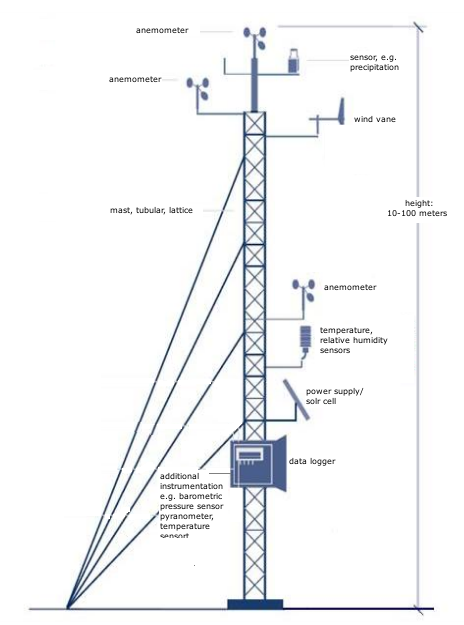
\includegraphics[width=0.5\textwidth]{figures/typical_met_mast.png}
\caption{Example of a typical met mast with various instrumentation, data logger, power supply and wiring. Typical instrumentation are cup anemometers or sonic anemometers, wind vanes, temperature, pressure and air density sensors, pyranometers and precipitation and humidity  sensors.}
\label{fig:met_mast}
\end{figure}






\section{Remote Sensing Instrumentation {\color{magenta}{Contributing author: ES}}}\label{sec:remote-sensing}




\section{Solar Radiation Sensors }\label{sec:solarradiation}


\section{Instrumentation on Met stations }\label{sec:metstations}


\section{SCADA Power Measurement Systems {\color{magenta}{Contributing author: JB}}}\label{sec:scadasystems}

\subsection{Wind Power SCADA systems }\label{subsec:scadasolar}

Suggested content:
\begin{itemize}
    \item Turbine anemometer (and issues)
    \item Relevant turbine SCADA parameters
    \item Relevant derived quantities (e.g. rotor effective wind speed, power available)
    \item ???
\end{itemize}

\subsection{Solar Power SCADA Systems }\label{subsec:scadawind}


%\section{}\label{sec:}

%\subsection{}\label{subsec:}

\chapter{Power Measurements for real-time operation }\label{ch:power_measurements}
{\color{magenta}{Contributing author: JB, RP? }}
%\\ \color{green} POST PUBLIC REVIEW VERSION\color{black}}
\label{ch:performanceassessment}

\noindent
\begin{tcolorbox}
\parbox{\textwidth}{
\emph{\textbf{Key Points}
\begin{itemize}
    \item Live power and energy data are a valuable input to very short-term forecasting systems, especially those with frequent updates and high temporal granularity
    \item Additional operational data such as Power Available signals, plant set-points, and availability are critical for robust forecasting and forecast evaluation
    \item The specification of power and energy metering should be factored into forecasting systems
\end{itemize}
}}
\end{tcolorbox}




\section{Live power and related measurements}
\label{sec:power_scada}

% Measurement location: wind turbine/solar panel, plant-level aggregation, connection point.

Real-time measurements of power production from wind and solar farms are are a valuable input to very short-term forecasting systems, those with lead-times of minutes to hours ahead. This and related data can also assist monitoring of plant availability which is important for operational forecasting. Real-time power data has the potential to significantly increase the accuracy of very short-term forecasts compared to those based on Numerical Weather Prediction and/or those which incorporate real-time meteorological data. Power measurements have the advantage of being the quantity that is being forecast and therefore not subject to errors when converting wind speed to power, for example. However, power production is affected by non-weather effects, such as control actions from system operators, which should be considered by forecasters.

Power production may be measured at multiple points between individual generators (individual wind turbines or PV panels) and the point of connection to the electricity network. In the majority of cases, the energy metered at the connection point and used in settlement of the electricity market is the quantity to be forecast. Accuracy standards for settlement meters are generally high, and live data are typically available to at least the plant and relevant electricity system operator. Power from individual generators or other points in a wind or solar park's internal network will be subject to losses so will not match the settlement meter. This data may however be utilised to improve forecasts.

Temporal resolution is an important factor when considering the use of live data in forecasting systems. Different users may be concerned with power/energy production on different time scales. Market participants' primary concern is energy in a given settlement period, which differ in length between countries/regions, and between financial products for energy and other services, such as reserve products. Settlement periods with 5, 15, 30, 60, 240 minute duration are common. System operators, on the other hand, may be more concerned with instantaneous power for balancing purposes, though in forecasting practice this may be approximated by averaging over a short time period or smoothing. Real-time data should be collected at the same or higher resolution than the user requires. Higher resolution data also enables more frequent updates to forecasts as new data becomes available more frequently.

A list of common measurements and their potential uses in forecasting systems is provided in Table~\ref{tab:power_variables}. In general, they are collected by the plant's Supervisory Control and Data Acquisition (SCADA) system, or by dedicated metering/monitoring devices that communicate with the electricity system and/or market operator.

\begin{table}[]
    \centering
    \caption{List of power-related quantities measured at wind (W) and solar (S) plants that have a role in forecasting and examples of how they may be used.}
    \begin{tabular}{|p{3cm}|c|p{4cm}|p{6.5cm}|} \hline
         Quantity & W/S & Location & Use \\ \hline
         Active Power & W\&S & SCADA or Connection Point & Input/feature in very short-term forecasting models, indicator of plant availability if combined with meteorological measurements \\
         Controller Set-point & W\&S & SCADA & Flagging curtailment and other control actions \\
         Capacity in operation & W\&S & SCADA & Scaling forecast based on available capacity \\
         Voltage & W\&S & SCADA or Connection Point & Flagging plant unavailability \\
         Status of breakers & W\&S & & Flagging plant unavailability \\
         Temperature & W\&S & Plant & Forecast input: PV efficiency, snow, icing \\
         Wind Speed & W & Turbine SCADA or Met Mast & Forecast input and quality control \\
         Wind Direction & W & Turbine SCADA or Met Mast & Forecast input and quality control \\
         Horizontal direct solar radiation & S & Plant & Forecast input and quality control \\
         Panel Tilt & S & Plant & Forecast input and quality control \\
         Sky images & S & Plant & Forecast input \\\hline
    \end{tabular}
    \label{tab:power_variables}
\end{table}


% {\color{magenta}{Measurements: active power, turbine/panel operational or not, maximum export/capacity, turbine/panel/plant controller set-point, power available/available active power. Net-load of PV/demand, larger PV require separate meters in some cases. Hilight challenges for embedded wind and solar without live data (and size threshold depends on system).}}

% {\color{blue}{Question: what is our aim with this section ? \\ My understanding is that there are grid codes and well defined ways of collecting data at TSO level. Is our aim to make suggestions to: (1)  TSOs on what may be missing or what is crucial from a forecasting perspective ? \\ (2) BRP to assist them in requesting specific power data from wind/solar famrs for the marketing and balancing ?}}
% {\color{magenta}{Yes, exactly.}}

\section{Power available signals}
\label{sec:power_available}

Power Available (PA) signals provide an estimate of the potential power that could be produced by a wind or solar plant if not constrained in any way. Constraints are typically reduced controller set-points issued by the plant or electricity system operator. PA is equal to active power under normal operation, or the power that could be produced if any constraints were lifted. Wind and solar plant typically produce PA signals internally for control purposes, and in some jurisdictions these are shared with electricity system operators.

Wind and solar power forecasts are typically configured to forecast the power that would be produced in the absence of constraints, which therefore corresponds to PA signals when such actions are in place. Furthermore, forecasts that take live power as an input should switch to taking PA as an input during constraints, or at least flag power data as corrupt during these periods.

\section{Measurement systems}

\subsection{Connection-point Meters}

The interface between a power plant and the electricity system, the so-called connection-point, is typically metered to a high degree of precision and used in electricity market settlement and provide a live feed to plant and system operators. The minimum precision of such measurements is usually dictated by network codes in a given region. For example, international standard IEC 62053-21 and IEC 62053-23 describe classes of active and reactive power meters, respectively. These standards are references in the Great Britain Balancing and Settlement Code, for example, where active power meter errors are required to be less than 1.5\% under normal conditions, or 2.5\% if the power factor is beyond 0.5 lag or 0.8 lead, or active power is below 20\% or rated import/export. It should be noted that these measurements may not match those recorded by plant plant SCADA systems (the topic of the next section) due to differences in equipment or location of measurement devices relative to the grid connection-point transformers and other electrical equipment.

Live power data is often streamed to plant and system operators and  available to control room engineers and their support systems and is often visualised along side forecasts to track out-turn relative to forecasts continuously. Live data is also a key input to very short-term forecasting systems with high temporal granularity, which is discussed in Section~\ref{sec:liva-data-so}. 

Energy is metered according to the duration of market settlement periods, which typically range from 5 to 60 minutes. As the volume of energy used in market settlement, predicting the volume of energy measured by these meters is the objective of the majority of forecasting systems, especially those used by market participants.

\subsection{Wind Power SCADA Systems }\label{subsec:scadasolar}
{\color{magenta}{Contributing author: JB}}{\color{blue}{ -- needs attention - more authors ? COM: 23.08.2021 still valid ?}}

Wind turbines routinely measure operational variables for their control and operation. Several of these are valuable in forecasting, particularly on the very short-term horizons if provided in close to real-time to forecasting systems. These are listed in Table~\ref{tab:power_varia}. However, it is important to note the limitations of these, in particular of the nacelle mounted anemometer and wind vane, which are impacted by the up-wind rotor, see Section~{\color{magenta}{cross-ref}} for more details. The sampling frequency if also significant. Typically 10-minute mean values are stored and communicated to control control centres, but higher resolution may be of value, particularly if maximising forecast accuracy on lead-times of 10-minutes or less is a high priority. Live feed of instantaneous active power can be valuable in very short-term forecasting, though it is important to treat both instantaneous power and power averaged over different time periods as distinct.


\subsection{Solar Power SCADA Systems {\color{magenta}{Contributing author: ?}}}\label{subsec:scadawind}

{\color{magenta}{JB has reached out to members of IEA PVPS 16 and Justin Sharp for input. Rui also offered to speak to contact and contribute here.}}
% John Z can contact Amber from CASIO with specific questions once we have a draft.

\subsection{Emerging technologies {\color{magenta}{Contributing author: ?}}}\label{subsec:scadawind}

The rapid evolution of energy systems requires forecasting systems to evolve with them. Some emerging issues are briefly discussed here.

Embedded wind and solar, that which is connected `behind the meter' is observed negative demand in many electricity systems. This poses a challenge as both the installed capacity, location, and power output of these generators may be unknown. Various actors be require forecasts of net-load with gross load and embedded generation disaggregated. In this case, a combination of net-load metering, meteorological observations, and wind and solar production data all add value to forecasting systems. Where the installed capacity is uncertain, satellite imagery may be employed to identify the size and location of wind turbines and solar panels.


% Suggested content:
% \begin{itemize}
%     \item Net-load metering and forecasting
%     \item Capacity estimation: net-load data, satellite images
%     \item Real-time monitoring: satellite data (radiation and wind), networks of measurement devices, partial metering and up-scaling
%     \item ???
% \end{itemize}



\section{Live power data in forecasting}
 \label{sec:live-data}

Live measurements of the quantity of being forecast are the most important inputs to any forecasting system on very short lead-times. Their recency and locality cannot be matched by modelling due to latency and epistemic uncertainty introduced by modelling, except in the case where live measurements are corrupted. In general, methods based on live data outperform NWP-based forecasts for lead-times shorter than 2--10 hours, depending on the specific of the target variable and reference NWP. State-of-the-art forecasting systems will combine both approaches for optimal performance at all lead-times, and may also include live data from multiple neighbouring measurement locations for added benefit.

In addition to live measurements of the forecast variable, operational data such as plant availability (e.g. proportion of turbines/PV panels in service) and control actions (e.g. curtailments) are also required as they change the nature of the power measurement. State-of-the-art forecasting systems will adapt to changing operational regimes and must be calibrated to predict the variable of interest to the user: what the actual power production is expected to be in the future, or, the the power production would be expected to be in the future if no control actions were in effect.  Forecasting systems must also be robust to missing data and able to either adapt to the loss of a live feed, or impute missing values.

% Robustness of data feeds/communication/etc?

% {\color{magenta}{Delays/latency in communications. Maybe a table of `issue|detail|impact'?}}

{\color{magenta}{JB to make illustration/example figure here.}}

\subsection{Specifics for producers of forecasts}
\label{sec:live-data-producer}

It is best practice for those who produce forecasts for internal use or to supply to  incorporate live data into their forecasting system for both continuous forecast verification (see Recommended Practice on Forecast Solution Selection) and production of very short-term forecasts. As discussed above, live data is a valuable input input to very short-term forecasting systems, and depending on the nature of forecast produce/service, may be necessary for post-processing to account for plant availability. Live data may also be included in forecast visualisation so that users may see recent history in the same figure as a forecast.


\subsection{Specifics for consumers/users of forecasts} 
\label{sec:liva-data-so}

Consumers/users of forecasts should be aware of whether their forecast provider is using live data when producing forecasts, especially for very short-term lead-times. Some of the benefit of including live data may be realised by rudimentary methods, such as blending live data with forecasts or simply visualising recent observations alongside forecasts. However, to maximise forecast performance it is recommended to employ an forecasting system of provider that leverages live data.



\chapter{Measurement Setup and Calibration }
%\\ \color{green} POST PUBLIC REVIEW VERSION\color{black}}
\label{ch:measurements}
{\color{magenta}{Contributing author: JZ, COM}}{\color{blue}{ -- needs cleanup and some decisions Table \ref{tab:requirements_on_instrumentaion},table \ref{tab:requirements_on_instrumentaion}, section \ref{subsec:selection_of_instrumentation}, section \ref{subsec:measurement-characteristics}, Table \ref{tab:pyranometer_classes}
}}
\color{black}
\noindent
\begin{tcolorbox}
\parbox{\textwidth}{
\emph{\textbf{Key Points}
\begin{itemize}
    \item Instrumentation Selection
                \begin{enumerate}
             \item Evaluation of the required data accuracy or uncertainty levels
            \item Cost-benefit analysis of instrumentation regarding quality and maintenance requirements
            \item Specification on redundancy levels
        \end{enumerate}
    \item Representativeness of Measurements
    \item Verification of correctness of installation and calibration
    \item Setup and Calibration Logging
    \item Maintenance Schedules of instrumentation
\end{itemize}
}}
\end{tcolorbox}

%\section{ TITLE {\color{magenta}{Contributing author: }}}\label{}
%\subsection{TITLE {\color{magenta}{Contributing author: }}}\label{}
\iffalse
\color{red}
Thoughts on this chapter (Corinna):
\begin{itemize}
    \item This is for commenting
    \item balblabla
\end{itemize}

\color{purple}
Changes made by COM: \\
blablabla
\color{black}
\fi

\section{Selection of instrumentation}\label{sec:instrumentation_selection}

{\color{blue}{Comments from SW (28.06.2021: also include comments on how representative the measurements of different instruments are}}

In this section we will describe best practice for the selection of instrumentation for forecasting applications of wind and solar projects. 
We focus in this description not on instruments, but rather on the requirements and necessary considerations for the selection of instrument classes that are appropriate for the pre-defined requirements. 

The first step in the selection procedure is the definition of requirements for the forecasting application. Table \ref{tab:requirements_on_instrumentaion} will provide typical forecasting applications and respective appropriate requirements. 

\begin{longtable}{  p{.20\textwidth} | p{.30\textwidth} |  p{.40\textwidth} }
 \caption{Forecast applications and respective requirements for appropriate instrumentation.}\\
 \hline
 \textbf{Forecast Application} & \textbf{Requirements for Wind} & \textbf{Requirements for Solar}\\ \hline
 \endfirsthead
 \textbf{} & \textbf{} &  \\ \hline
 \endhead
System Operation Forecasting &  Class A & Secondary Standard\\ 
Park control & Class A & Secondary Standard\\ 
Trading & Class B & First Class \\ 
Park Monitoring & Class S & Second Class \\ 
.. & .. & .. \\ 
.. & .. & .. \\ \hline
  \label{tab:requirements_on_instrumentaion}
\end{longtable}

The classes for wind projects are defined in 

\subsection{Selection of instrumentation for wind projects}\label{subsec:instrumentation_selection}

{\color{red}{Comments from COM (21,08,2021):I do not think that this is the goal of our RP here and how the selection of instrumentation should be in our context of real-time forecasting!!!}} \\
\sout{The selection of instrumentation for an operational wind farm should be selected to ensure (1)  its best performance  and (2) reliable power generation. The profitability is connected to the performance of the wind turbines and has to be monitored, as well as each wind turbine and the wind farm in it's entirety needs to be controlled by implementing SCADA systems.}

{\color{green}{Comments from COM (22.08,2021): SUGGESTION\\
The selection of instrumentation of meteorological measurements for forecasting applcations of operational wind farms should be selected to ensure (1) an independent source of measurment to the power generation and (2) a good fit to the power generation of the wind farm. 
}}

In other words, there is a need for appropriate measurement equipment in the sense of: 
\begin{itemize}
    \item Accuracy 
        \begin{itemize}
            \vspace{-0.2cm}\item appropriate quality of instrumentation
           \vspace{-0.2cm} \item uncertainty evaluation of instrumentation
        \end{itemize}
    \item Reliability
        \begin{itemize}
            \vspace{-0.2cm}\item correct installation of instrumentation
           \vspace{-0.2cm} \item correct calibration of instrumentation
            \vspace{-0.2cm}\item redundant setup of instrumentation and logging
        \end{itemize}
    \item Availability
        \begin{itemize}
            \vspace{-0.2cm}\item instruments being redundant
            \vspace{-0.2cm}\item loggers being fail safe
        \end{itemize}
    \item Weather resistant and safe
        \begin{itemize}
            \vspace{-0.2cm}\item meet local requirements of climate
            \vspace{-0.2cm}\item meet local requirements of landscape
            \vspace{-0.2cm}\item meet safety requirements (e.g. flight safe in case of met masts at hub height)
        \end{itemize} 
\end{itemize}


\subsubsection{Components of a wind measurement systems {\color{blue}{Comments from COM (21.08.2021: moved to section \ref{sec:wind_instrumentation}}}}

This list provides a general guidance of the four most important aspects that need consideration in the selection process of instrumentation for real-time forecasting applications. 

It is important for any authority (e.g. TSO, DSO, ultility or balance responsible party) to go through these aspects, when setting requirements for the instrumentation. Dependent on these aspects, there are standards available that guide the wind farm operators to the instrumentation that is appropriate for the requirements set out by the authority. 

In this recommended practice guideline, we therefore focus on the procedure and instrument classes rather than the individual instrumentation, as these are handled by available standards (see section \ref{sec:met_standards} for a description of the applicable standards). 

For wind measurements, there is a principle of three tiers of instrument standard class available that are dependent on the requirements to accuracy and reliability and are also associated with different cost levels. It is therefore recommended to define the requirements first, before requiring a specific instrumentation quality standard. 

The ``GUIDE TO INSTRUMENTS AND METHODS OF OBSERVATION - VOLUME I''\cite{wmoguide2018} defines important requirements for meteorological instruments to:

\begin{enumerate}
    \vspace{-0.2cm}\item Simplicity of design which is consistent with requirements
    \vspace{-0.4cm}\item Durability
    \vspace{-0.4cm}\item Convenience of operation, calibration and maintenance
    \vspace{-0.4cm}\item Acceptable cost of instrument, consumables and spare parts
    \vspace{-0.4cm}\item Safe for staff and the environment
\end{enumerate}

It is recommended that authorities refer to the classification of  instruments in their requirements or provide accuracy limits. 

The IEC 61400 standard \cite{iec61400-12-1-2005}, for example, privides information on anemometers according to class A, class B or class S types, where the classes of instrumentation are dependent on the terrain structure defined in Annex B of the standard. In areas with complex terrain, the class B standard requires e.g. specific setup of instrumentation to accomodate the influence of turbulence from varying terrain etc. 
The class S is associated with specific requirements, ``where  the  influence  parameter  ranges  are  restricted  to  allow  for  the  specified  accuracy  of  the  anemometer.'' \cite{iec61400-12-1-2005}. Manufacturers of wind instrumentation that sell instruments for wind projects provide information about the class of instrumentation to make it easy for wind farm owners to purchase the approapriate instruments. 


The following table describes the main and applicable types of instrument classes in their respective environments. 

\begin{table}[h!]
    \caption{Instrument classes for various environements.{\color{red}{Comments from COM (21.08.2021:NEEDS DISCUSSION and more info}}}
    \centering
    \begin{tabular}{p{4cm}| p{7cm} | p{3cm}}
     \textbf{Environment type}  & \textbf{Environment description} & \textbf{Instrument class} \\ \hline 
     Standard terrain  & Flat terrain with few obstacles & class A \\
     Complex terrain   & varying heights and many obstacles  &  class B\\
     offshore          & wave and current driven turbulence \\ salty air & classe S \\
     ... & & \\
    \end{tabular}
    \label{tab:initial_considerations}
\end{table}



\subsection{Selection of instrumentation for solar power plants}\label{subsec:selection_of_instrumentation}




In the IEA PVPS handbook for the collection and use of solar resource data \cite{nrelhandbook2021} the authors present recommendations for the selection of the instruments. These recommendations also apply for the real-time applications. Depending on the solar technology used different radiation components must be measured. The requirements for fixed monofacial PV or thermal collectors, bifacial PV, concentrating systems and tracked non-concentrating PV are different. Besides radiometers also further meteorological parameters must be measured as stated above. For selecting the instrumentation, the user must also evaluate the required data accuracy and consider the effort necessary to operate and maintain the measurement system. Specifically, the most accurate instrumentation should not be purchased, if the project resources cannot support the maintenance required to ensure measurement quality consistent with the radiometer design specifications and manufacturer recommendations. 
Various radiometers of the same type should be considered for big power plants and are also helpful to ensure a higher data quality. The number of required instruments for PV parks of different peak power is given in IEC 61724-1 along to further requirements on instrument accuracy, maintenance and data logging. Multiple radiometers within a project location and/or providing for the measurement of all three solar irradiance components (GHI, DHI, and DNI) can greatly enhance opportunities for post-measurement data quality assessment.

To summarise, the following considerations should be taken in the selection process:

\begin{enumerate}
    \item Evaluation of the required parameters, data accuracy or uncertainty levels
    \item Cost-benefit analysis of instrumentation regarding quality and maintenance requirements
    \item Specification of number of instruments
\end{enumerate}
   

{\color{red}{Comments from COM (21.08.2021:SUGGESTION --- NEEDS DISCUSSION and ADDED INFORMATION\\

For the selection of pyranometers, the ISO 9060 standard "Solar energy - Specification and classification of instruments for measuring hemispherical solar and direct solar radiation"\cite{ISO9060}, also used and approved by the WMO, separates between 3 classes of instruments. 

\begin{enumerate}
  
    \vspace{-0.2cm}\item Secondary Standard
    \vspace{-0.2cm}\item First Class
    \vspace{-0.2cm}\item Second Class
\end{enumerate}


The following table provides a summary of the applicability of these classes in solar energy forecasting. 
}}
\begin{table}[h!]
    \caption{Pyranometer classes for various requirements. {\color{red}{Comments from COM (21.08.2021:SUGGESTION --- NEEDS DISCUSSION and ADDED INFORMATION}}}
    \centering
    \begin{tabular}{p{6cm} | p{4cm} | p{4cm}}
    \toprule
     \textbf{Requirements}  & \textbf{Instrument class}     & \textbf{Instrument description} \\ \hline 
     Meteorological or Energy forecasting/ modelling &  Secondary Standard & Scientific quality and highest accuracy \\
     & & & \\ 
     Measurements for high level monitoring & First Class & Good quality \\
      & & & \\
     Economic solutions for routine measurements & Second Class & Medium quality \\
     ... & & \\
    \end{tabular}
    \label{tab:pyranometer_classes}
\end{table}


\subsubsection{Components of a PV measurement system}

\subsection{Measurement Characteristics of Different Technologies} \label{subsec:measurement-characteristics}

{\color{magenta}{Discussion of conceptual differences in measurements from anemometers on met masts (point measurements), remote sensing devices (lidar,sodar - which are some type of volume average) and nacelle mounted anemometers (very representative of height and location of turbines but obstructed). \\
}}
{\color{blue}{Questions:\\ Under 4.1.3 (Measurement Characteristics of different technologies), do we want to include solar-related measurements in this?  Ground-based pyranometer vs satellite-based estimate?
}}

\subsubsection{Measurement Characteristics of Lidars}

\textbf{Measuring Laminar Low Level Jets}

An advantage of the remote sensing device's ability to measure the wind profile is it's ability to "measure" low level jets [Kelly et al 2014] that can have significant influence for the power production forecasting. The low level jets are a meteorological phenomenon that is a well-known and extensively researched topic in meteorology since the 1950s [e.g. Blackader, 1957, Zhang, 1996] and has been a topic in wind energy research since forecasting started. 

Recent progress with the help of wind profilers (SODAR, LiDAR) as well as comparisons with a 120m mast has been made in the Lamar Low Level Jet Program, reported by Kelly et al [2014] over a 1-year period. 


\subsubsection{Lightning effects on instrumentation}

It is a know phenomena (e.g. Kelly et al [2014]) that lightning can cause high frequency noise contamination to instruments. 
This is applicable for: 
\begin{itemize}
    \item Remote Sensing instruments (LIDAR, SODAR, RADAR)
    \item sonic anemometers
\end{itemize}

In the case of LIDAR or SODAR lightning contaminates the signal processing with echoes. Such echo reflections can make it impossible for the signal software to process the signal correctly and hence the data cannot be used.
In resource assessment of research projects, such noise can be corrected and the data re-processed to provide valuable data. In Real-time this is not possible. 

In the case of sonic anemometers, high-frequency noise contamination disturbes the sonic signals of wind velocity and temperature and usually makes the data unusable.

\textbf{Maintenance and mitigation methods}
These examples shows that the maintenance and upgrades of software to make use of fixes in the signal processing algorithms of the devices are a key technical requirement for real-time use of the devices, or alternatively that the raw data needs to be sent and the processing takes place where the data is used. 

Therefore, we can conclude that the reliability of any measurement device in real-time operation requires a maintenance schedule to be a technical requirement in order for it not to deteriorate. If this is done, the remote sensing instruments as well as sonic anemometers have proven to provide reliable time series of wind speeds and gusts in general conditions. 





\section{Location of Measurements}\label{sec:location-of-measurements}
        
{\color{magenta}{Comment SW,  COM (21.08.2021): Add an introductory paragraph under 3.1 to describe the issue - that the objective is to make measurements that are well correlated to the power generation (wind or solar) and what issues affect that correlation.}}



{\color{blue}{Comments from John (21.04.2021:\\
Questions: \\
\begin{itemize}
\item Do we know of a guidance that has been written for the horizontal placement of an anemometer or sodar/lidar or solar maesurement for forecasting applications? \\ 
\item  Should the location be well-correlated with the power production from the facility. But what guidance should be provided for that?  \\
Prevailing upstream direction at the roughly the hub height for wind facilities is basic guidance? \\ 
\item  In simple terrain that might be OK but in more complex terrain what guidance can we give?\\
\end{itemize}

More comments from John (JZ) 13.6.2021:

Done: background work on collecting academic papers that have been published on how to determine the most representative \\
 -- location for a single (or two or more..) \\

 --wind measurement(s) to have the highest correlation with the power\\ generation.  
 
 Are there more/any quantitative work that has been done on this?


Intuitive general principles - i.e.\\ 
 (a) place it in the prevailing upstream direction,\\ 
 (b) avoid locations that are frequently in wakes,\\ 
 (c) avoid being near terrain features or roughness elements that are not typical of the overall generation facility etc. 
 
 But can we say more than this? Or show a quantitative example?  Or reference one or more papers?  
 
 What do we say about irradiance measurement location for solar - at the plant centroid? 

Similarly for the vertical location (4.2.2) - measurements near hub height and/or ver

}}







The WMO Report Nr. 55 \cite{wmoreport1993} describes the site and instrumentation selection as a 6-tier problem:
\begin{enumerate}
    \vspace{-0.2cm}\item selection of a suitable site
    \vspace{-0.4cm}\item correct exposure of instruments
    \vspace{-0.4cm}\item determination of the area of representativeness of measurements
    \vspace{-0.4cm}\item description of the site and its facilities
    \vspace{-0.4cm}\item homogeneity of the meteorological/climatological data*
    \vspace{-0.4cm}\item access to information* 
\end{enumerate}

The last two tiers require international collaboration to ensure measured data can be compared and the precision and accuracy of the measured data follows a common understanding for the use in models and methods to improve or interpret model results. We will not deal with these aspects in this document, but want to bring these topics to anyone dealing with measurements to his or her awareness and that the meteorological community has solved these critical problems by establishing international data networks to provide modellers, researchers, instrument developers and end-users the possibility to progress and exchange information. 

The fifth tier deals deals with the lack of international homogeneity on measuring standards that has been a problem in meteorology and can also be observed in wind and solar projects on an international scale. If data measuring standards are not international, it is difficult to obtain homogenity in data and thus models and methods, where such data are used. 


{\color{magenta}{comment SW: I think the following text should be deleted. this belongs to the section "selection of instruments"}\ref{subsec:selection_of_instrumentation}}
\\
{\color{magenta}{One of these problems are the accuracy of instruments. It is very important to define the purpose of measuring and the expectation on the accuracy of the measured quantity. For example, if the accuracy of an instrument is $\mp{0.3}$ and the target is an accuracy of 0.1, neither the instrument nor the measured quantity can provide a representative picture.  }}z







%\subsection{Location of Instrumentation}\label{subsec:selection-of-location}
{\color{magenta}{ Discuss location specifics regarding terrain differences etc.}}
{\color{magenta}{ comment SW 210715: I removed the title "location of instrumentation". I think it is much easier to write and to read if the following text is in the section location of measurements}}
%REPRESENTATIVNESS ???

%\subsection{Measurement Characteristics of Different Technologies}  ---> moved to section 4.1 \ref{subsec:instrumentation_selection}---> search for \ref{subsec:measurement-characteristics}

The Guide for WMO Guide for Meteorological Measurements \cite{guidewmo2018} (``WMO Guide 8'') contains in it's \textit{ANNEX 1.D. SITING CLASSIFICATIONS FOR SURFACE OBSERVING STATIONS ON LAND} information about siting of instrumentation to ensure representativeness. The guide covers all meteorological instrumentation that are relevant for wind and solar projects and operation. 

The WMO Guide 8 states that ``..the environmental conditions of a site may influence measurement results. These conditions must be carefully analysed, in addition to assessing characteristics of the instrument itself, so as to avoid distorting the measurement results and affecting their representativeness..'' and recognises that ``...there are sites that do not respect the recommended exposure rules''. 

Out of these conditions, the WMO has developed a classification with 5 classes to ``help determine the given site’s representativeness on a small scale (impact of the surrounding environment)'' and help to better take their exposure rules into consideration. 

The classes can be summarised to:
\begin{enumerate}
    \vspace{-0.4}\item class: reference site
    \item class: additional uncertainty added by siting through a value relative to the previous class 
    \item class: additional uncertainty added by siting through a value relative to the previous class 
    \item class: additional uncertainty added by siting through a value relative to the previous class 
    \item class: Nearby obstacles create an inappropriate environment for a meteorological measurement that is intended to be representative of a wide area
\end{enumerate}


The most relevant and useful rules to consider also for wind and solar projects are the following:
\begin{itemize}
    \item The classification takes place per instrument, not per site as a whole
    \item The rating of each site should be reviewed periodically as environmental circumstances can change over a period of time
    \item A complete update of the site classes should be done at least every five years
    \item An uncertainty due to siting has to be added in the uncertainty budget of the measurement
    \item The primary objective of the classification should be to document the presence of obstacles close to the measurement site
\end{itemize}


For solar power plants the location of the instruments is of importance as the irradiance can vary within the park due to clouds or shading. Soiling, albedo, wind speed and temperature can also vary strongly. For PV plants recommendations on the number and position of the instruments can be found in IEC 61724-1. Sensors should be distributed over the whole area of the power plant and of course not concentrated at a single site. The location of the instruments should be selected as representative for the covered sections of the power plant. For radiometers mounted on the front side of the PV modules shading should be avoided. For rear side instruments and albedo measurements the number of required radiometers depends also on the variability of the ground surface. For rear side sensors multiple sensors are recommended at different positions on the module, as the illumination profile is not uniform.


\section{Installation of measurement station {\color{blue}{needs attention}}}\label{sec:installation-veification}

{\color{magenta}{comment SW 210715: I removed the word "siting" from the title. This should be all together discussed in the section on instrument location. I commented out the text summarizing the WMO info here as it did seem helpful to me not even for the previous section on location. I assume a general text refering to the CIMO guide will open the section. }}
 
 Specific information on the installation of radiometric stations can be found in \cite{nrelhandbook2021}.
 
%Siting and installation of measurement stations, or ``Automatic Weather Stations'' (\cite{guidewmo2018}) should, according to the WMO Guide \cite{wmoguide2018} be designed so that representative measurements (or observations) can be taken according to the type of station involved. In Meteorology, the distinction is on weather scales such as meso-scale (10-100 km) or synoptic scale ( ~1000km) or aviation observation stations (local). A station in a meso-scale network should make observations to meet meso-scale requirements and an aviation station should describe the conditions specific to the local (aerodrome) site . The WMO Guide further requires that the most stringent requirement will dictate the precise location of an observing site and its associated sensing instruments, where stations are used for several purposes, for example, aviation, synoptic and climatological purposes. A detailed study on siting and exposure is published in WMO (1993).

%%% 

{\color{red}{COM: comment 21.08.2021: I have removed the siting figure from the WMO guide as I think we should not go into this detail, but rather point to the appropriate standards that define everything and rather discuss, what are appropriate reuqirments for real-time forecasting applications}}.

\iffalse
\begin{figure}
    \centering
    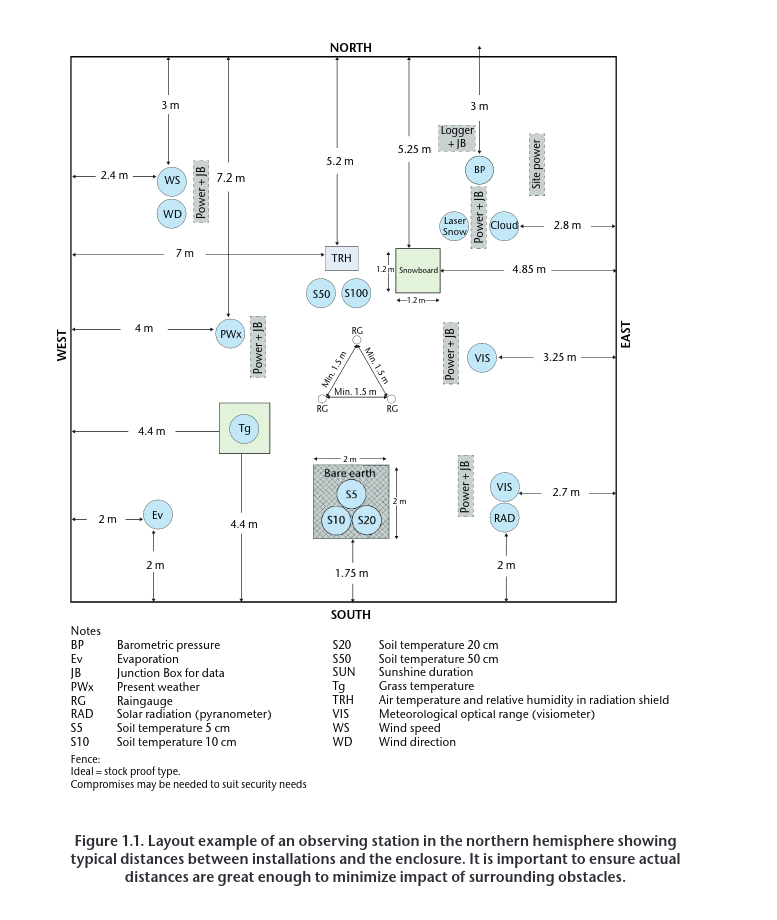
\includegraphics[width=\columnwidth]{figures/screenshots/wmo_nr8_siting.png}
    \caption{Layout example of an observing station in the northern hemisphere showing typical distances between installations and the enclosure . It is important to ensure actual distances are great enough to minimize impact of surrounding obstacles. \copyright WMO Guide to Instruments and Methods of Observation \cite{guidewmo2018}}
    \label{fig:decisionsupporttool}
\end{figure}
\fi

The exposure rules say that...



\subsubsection{Calibration and Correction methodologies for wake effects and yaw misalignment}\label{subsubsec:calibration_and_correctio}

\textbf{Nacelle Anemometers}\\
\cite{Jing2020} for nacelle anemometers
%abstract = {For most wind turbines, blade wakes affect the measurement of nacelle anemometer, result in the inconsistency between nacelle wind speed (NWS) and free stream wind speed, which seriously affects the power forecasting and performance evaluation of wind turbine. This paper proposes a data-driven method to analyse the wake effect on nacelle anemometer. At first, we use Relevance Vector Machine to establish a site calibration model between Lidar wind speed (LWS) and NWS. After that, we can use the calibrated LWS to replace the free stream wind speed, and wake effect on nacelle anemometer can be evaluated by comparing the calibrated LWS and NWS. Then, Wind Turbine Power Curve (WTPC) is applied to make a detail analysis of wake effect on nacelle anemometer. The experimental results show that wake effect accelerates the air velocity behind the impeller. Therefore, WTPC fitted by NWS is “lower” than the real one. However, SCADA system overcorrects the wake effect, thus WTPC fitted by SCADA data is “higher” than the real power curve.}
%This paper proposes a site calibration model based on RVR, it has good performance compared with other typical site calibration methods. Accordingly, we can analyse the wake effect by comparing the LWS and NWS. The experimental results show that when the wind speed exceeds 6 m/s, blade wakes accelerate the air velocity behind the impeller, thus the average value of NWS is about 3\% higher than FSWS for power generation. Due to the wake effect on nacelle anemometer, WTPC fitted by NWS is 8\% “lower” than the real power curve. On the contrary, SCADA system overcorrects the NWS, and WTPC fitted by SWS is about 60\% “higher” than the real one. In the further study, we can use the same method to evaluate the wake effect in higher wind speed range.

\textbf{Scanning Lidars}\\
\cite{Held2019} have developed a method to detect wakes in the inflow of turbines using nacelle lidars and developed a correction method. 
%Nacelle-mounted lidar systems offer the possibility of remotely sensing the inflow of wind turbines. Due to the limitation of line-of-sight measurements and the limited number of focus positions, assumptions are necessary to derive useful inflow characteristics. Typically, horizontally homogeneous inflow is assumed which is well satisfied in flat, homogeneous terrain and over sufficiently large time averages. However, it is violated if a wake impinges the field of view of one of the beams. In such situations, the turbine yaw misalignment measurements show large biases which require the detection and5correction of these observations. Here, a detection algorithm is proposed based on the spectral broadening of the Doppler spectrum due to turbulence within the probe volume. The small-scale turbulence generated within wake flows will typically lead to a significantly larger broadening than in the ambient flow. Thus, by comparing the spectral widths at several locations,situations, where a wake is impinging the field of view of one or more beams can be identified. The correction method is based on an empirical relationship between the difference in turbulence levels at distinct beams and the difference in wind10direction derived from the lidar and the real wind direction. The performance of the algorithm is evaluated in a field experiment identifying all wake situations, and thus, correcting the lidar derived wind direction



 
\section{Maintenance and Inspection Schedules }\label{sec:maintenance-schedules}
The maintenance of the radiometers is often challenging. IEC 61724-1, ASTM G183 and ISO TR9901 recommend maintenance and inspection tasks including
\begin{itemize}
    \vspace{-0.2cm}\item cleaning
    \vspace{-0.4cm}\item levelling/tracking
    \vspace{-0.4cm}\item ventilation 
    \vspace{-0.4cm}\item desiccant
    \vspace{-0.4cm}\item general instrument status incl. cables
    \vspace{-0.4cm}\item and the quality control of the acquired data sets. 
\end{itemize}

    Also the intervals for the different tasks are given. With modern radiometers, and professional installation of the instruments, the task that has to be performed most frequently at the station itself is the cleaning of the sensors. The recommendations for cleaning are between daily (ISO), daily inspection and at least weekly cleaning (ASTM) and weekly cleaning (IEC). In fact the required maintenance frequency depends on the site, the instruments and the accuracy requirement as discussed in \cite{nrelhandbook2021}.  The quality control of the data must also be performed frequently as discussed above. Further information o the maintenance and inspection of solar measurement stations can be found in \cite{nrelhandbook2021}.


%\section{ TITLE {\color{magenta}{Contributing author: }}}\label{}
%\subsection{TITLE {\color{magenta}{Contributing author: }}}\label{}


\subsection{Documentation of setup, calibration, operation}\label{sec:logging-of-calibration}
{\color{blue}{Comment from SW (25.06.2021:  separate subsection seems too much.}}

The United States Environmental Protection Agency (EPA) provides a “Meteorological Monitoring Guidance for Regulatory modelling Applications” \cite{EPA2000} provides recommendations for  reporting for all main meteorological variables used in meteorological modelling.



\chapter{Assessment of Instrumentation Performance }
%\\ \color{green} POST PUBLIC REVIEW VERSION\color{black}}
\label{ch:performanceassessment}
{\color{magenta}{Contributing author: COM, AK }}{\color{blue}{ -- needs attention  }}

\noindent
\begin{tcolorbox}
\parbox{\textwidth}{
\emph{\textbf{Key Points}
\begin{itemize}
    \item All performance evaluations of potential or currently used instrumentation
    \item B...
    \item C...
    \item D...
\end{itemize}
}}
\end{tcolorbox}


The quality of measured data that is supposed to be used in real-time applications is of immense importance. Modern technologies to assimilate measured data into forecasting models usually have automatic algorithms that blacklist data that is out of range or in other ways suspicious, because bad data is often worse for the forecast model than no data. 

While low quality data can be compensated with longer collection periods or in general longer time-series for non real-time applications such as plant assessment and configuration, resource assessment, etc\., this is not possible in real-time environments, where the data has to be quality checked at the time of retrieval and processed or dismissed. 

Quality control and clear assessment criteria are therefore important tools for the success of the application using real-time measurements. 

In this chapter, we will describe challenges and mitigation strategies for the measurement data processing and quality control. 



\section{Measurement Data Processing {\color{blue}{needs attention}}}\label{sec:dataqa}



\subsection{Known issues of nacelle wind speeds and mitigation methods}

From a theoretical perspective, it can be expected that wake effects from the rotating blades are strongest at high speeds and low speeds that affect the mean wind flow, but not so much the correlation in the "normal" operating range. When plotting nacelle anemometer measured data in a scatter plot, where the linear relationship is strong in the range 3-12m/s and along the linear part of the power curve, this becomes most apparent. Below cut-in and above the wind speed where the power curve gets flat, the linear relationship does not hold any more. It has also been shown with frequency distributions that met mast anemometers produce an approximate Weibull distribution, where nacelle mounted instruments often produce strong biases at the lower wind speeds affected by wake effects.

This is due to 2 effect:
\begin{enumerate}
    \item wake effects from rotating blades
    \item Yaw misalignment of wind turbine
\end{enumerate}

In order to make use of nacelle mounted instrumentation corrections are necessary. The problems associated with these known issues are described in the following together with possible correction methodologies. 

\subsubsection{Wake effects from rotating blades}
Drechsel et al. [2012] found out that the wake effects of nacelle measured wind speeds are highest up until the cut-in wind speed and above approximately 10m/s, where the power curve starts getting flat.
Allik et al. [2014] found out in a study with nacelle mounted cup anemometers, nacelle mounted sonic anemometers and a reference met mast that the mean of the three measurements did not coincide very well. The nacelle wind speed measurements, due to the wake effects of the blades, have a much lower mean. The correlations however were strong between cup anemometer and met mast anemometer and even stronger between sonic anemometer and met mast readings within the range of 3-12m/s. 

Jing et al. \cite{Jing2020} also found that blade wakes affect the measurement of nacelle anemometer, result in the inconsistency between nacelle wind speed (NWS) and free stream wind speed, which seriously affects the power forecasting and performance evaluation of wind turbine.



\subsubsection{Yaw misalignment of wind turbine}

Held et al. \cite{Held2019} reports that due to the limitation of line-of-sight measurements and the limited number of focus positions of a scanning Lidar, assumptions are necessary to derive useful inflow characteristics at the turbine nacelle. The horizontally homogeneous inflow assumption is violated, if a wake impinges the field of view of one of the Lidar beams. In such situations, the turbine yaw misalignment measurements show large biases which require the detection and correction of these observations.



\subsection{Application of nacelle wind speeds in Real-time NWP Data Assimilation} \label{subsec:nacelle_wind_speeds_in_nwp_data_assimilation}

The only recorded project to date that carried out dedicated real-time studies with nacelle wind speeds in a real-time forecasting environment so far is the US Department of Energy funded “Wind Forecasting Improvement Project” (WFIP). The project had a demonstration phase of 1-year and used 410 nacelle wind speeds for the data assimilation of NOAAs models [Wilzcak, 2014, Marquis, 2014]. 

One of the main findings in the experiment was that the nacelle wind speeds were contaminated too much by wake effects to be useful as individual measurements. Due to the constraints in the data assimilation techniques, it was important to find a strategy that made it possible to use the raw data from the cup anemometers. The research team of NOAA found that the best way to handle the contaminated data was to average the individual turbine data per wind farm and then blacklist those measurements that were outside the range of 2 standard deviations from the mean of the wind farm. This is a reasonable constraint to ensure that measurements contaminated by wake effects will not be passed into the assimilation program. 

Additionally, the measurements were averaged over the nearest model grid point in the numerical weather prediction model. By doing this, it was possible to remove systematic biases and make use of the direct outcome of the model at the grid points. 

To summarise, the strategy to use all 411 nacelle measured wind speeds at 23 wind farms has been: 

\begin{itemize}
    \item averaging wind speed measurements over each wind farm
    \item blacklisting measurements that were more than two times a STD from the mean
    \item interpolating and averaging at the nearest grid point of the NWP model
    \item BIAS correcting at the model grid points
\end{itemize}


The advantage of this approach is that wake effects are smoothed out through the averaging within the wind farm and averaging at the NWP model grid points ensures that bias corrections are brought forward to the model result, i.e. the wind power forecast. In this way, it could be demonstrated that nacelle wind speeds can become useful signals seen from a general forecasting perspective.  


Pinson and Hagedorn \cite{PinsonHagedorn2012} used a different path to reduce uncertainty of the 633 meteorological stations with cup anemometers that they compared to model results. Their assumption was made according to the recorded uncertainty of unbiased state of the art anemometer uncertainty, which is a standard deviation of around 0.5m/s. It was shown that this was a reasonable and valid assumption. However, it is not known how much this assumption is dependent on the number of measurement units and their distribution. Therefore, such assumptions must be considered with care. 



\section{Uncertainty of instrumentation Signals }\label{sec:instrumentuncertainty}

In section \ref{} it was described that requesting uncertainty measures from instrumentation in real-time is unrealistic, but that a standing data value that is determined at the setup/calibration of the instrument and provided as part of the standing data, might be feasible.
{\color{blue}{comment SW 210715: This first sentence should be changed! I believe we must provide some uncertainty even with the live data. I think real time data is provided with uncertainty in many cases, It is difficult but can be done. }}
In that way, the instrument specific uncertainty could be accounted for in the handling of measurements. 

\textbf{Alternative instrumentation signal uncertainty estimations}
One alternative is to carry out an uncertainty estimation with e.g. the Monte-Carlo method described in \cite{jcgm2011} (pp23-33). 

Another alternative is to add a mean uncertainty value to raw measurements, as applied by Pinson and Hagedorn \cite{PinsonHagedorn2012} in an experiment over Ireland and Denmark with wind measurements from standard met masts [Pinson and Hagedorn, 2012 p7]. 

If a more standardised technical requirement is desirable, the JCGM guides \cite{jcgm2008,jcgm2008a,jcgm2009, jcgm2011,jcgm2012} offer a valuable general source, also applied in meteorology and oceanography. In that way, a harmonisation of "best practices" with these directly related real-time disciplines can be achieved. In fact, the guides do not only consider the measurand as a physical quantity, but also provide guidance to the conceptual design and the theoretical analysis of measurements and methods. 


%\section{Uncertainty of Measurements}\label{sec:measurementuncertainty}
%{\color{blue}{Comment from SW (25.06.2021:I think we can remove this section. as there is already a section on uncert. of signals.}}

\section{Quality control of measurements for real-time use}\label{sec:quality_control}

{\color{blue}{Author: COM -- needs more authors/discussion}}




{\color{blue}{Comment from COM (27.06.2021:
In Meteorology (see e.g. \cite{Lucio2018,Lucio2018a}:
(1) data management errors:
    - data transcription and collection
    - errors that occurred during data manipulation (e.g. duplication of data sequences)
    - standardization of practices (e.g. measurement units, reference times) 
    
(2) measurement errors: 
    - temporal or spatial consistency in the data
    - errors produced at the moment of sampling as a result of :
        - instrumental malfunction
        - calibration
        - exposure problems

---------------------------------------------------------

\textbf{Comments from COM: 19.08.2021}

---------------------------------------------------------

I like EPA's definition of QC and QA and would like to discuss this -- with the goal in mind that we are aiming to provide a practical guideline! \\

The EPA's Meteorological guidance for the use of observational data (see \url{https://www.epa.gov/sites/default/files/2020-10/documents/mmgrma_0.pdf} )says the following:  
Quality Assurance/Quality Control (QA/QC) procedures are required to ensure that the data collected meet standards of reliability and accuracy.\\  

- \textbf{Quality Control (QC)} is defined as those operational procedures that will be routinely followed during the normal operation of the monitoring system to ensure that a measurement process is working properly. These procedures include periodic calibration of the instruments, site inspections, data screening,data validation, and preventive maintenance.  The QC procedures should produce quantitative documentation to support claims of accuracy.  \\

- \textbf{Quality Assurance (QA)} is defined as those procedures that will be performed on a more occasional basis to provide assurance that the measurement process is producing data that meets the data quality objectives (DQO).  These procedures include routine evaluation of how the QC procedures are implemented (system audits) and assessments of instrument performance (performance audits).\\

The QAQC procedures should be documented in a Quality Assurance Project Plan (QAPP) and should include a "sign-off" by the appropriate project or organizational authority. The QAPP should include the following [63]: 

1.  Project description - how meteorology is to be used 

2.  Project organization - how data validity is supported 

3.  QA objective - how QA will document validity claims 

4.  Calibration method and frequency - for meteorology 

5.  Data flow - from samples to archived valid values 

6.  Validation and reporting methods - for meteorology 

7.  Audits - performance and system 

8.  Preventive maintenance 

9.  Procedures to implement QA objectives - details

10.  Management support - corrective action and reports \\

It is important that the person providing the QA be independent of the organization responsible for the collection of the data and the maintenance of the measurement systems. 

Ideally, this person should be employed by an independent company.  There should not be any lines of intimidation available to the operators which might be used to influence the QA audit report and actions.  With identical goals of valid data, the QA person should encourage the operator to use the same methods the QA person uses (presumably these are the most comprehensive methods) when challenging the measurement system during a performance audit. 

\textbf{When this is done, the QA task reduces to spot checks of performance and examination of records thus providing the best data with the best documentation at the least cost.}\\


\textbf{For us this recommendation could look like this:} \\
\textbf{1. Project Description and organisation}\\
...    - how measurements are to be used\\
...    - how measurement signals are collected and stored\\
...    - how data validity is defined and reported\\
...    - QA objective and how QA will document validity claims\\
    
\textbf{2. QA procedure and monitoring} \\
...    - Provision and Monitoring is done by an agent independent of the end-user and the data provider (e.g. forecaster, IT consultant)
...    - Regular data validation and verification \\
...    - Performance monitoring and Reporting\\
...    - Corrective Actions according to Reports\\




}}

The purpose of quality control of measurements is to ensure that data can be used for forecasting 

There are 2 time horizons for the quality control: 
\begin{enumerate}
    \item QC in real-time forecasting at the time of receipt; ``black- and white listing''
    \item QC in historic mode: \\ quality control of a specific time interval of data such as a day, a month or one or more years for resource assessment, performance monitoring, model/forecast training/tuning etc. 
\end{enumerate}
{\color{blue}{comment SW 210715: Why should we define that real time QC is a black and white listing? One could also imagine another category of suspicious data that is used but assuming a higher uncertainty than normal so that it influences the forecasts less. At this point I wouldn't exclude such an option.}}
{\color{green}{comment COM 210726: Agree, but it needs to be specified more here. E.g. that in extreme events, suspicious data often show the real happening. Today, I think this is not practices very much to keep algorithms robust, but we should mention that the optimal use is to include the uncertainty...}}



\section{General data quality control (QC)}
repeated values, values out of range limits, formatting of data file/decoding error, consistency of time stamps/chronologically, time averaging definition, site coordinates, instrumentation identification

\subsection{Accuracy and Resolution Limits}
Table \ref{tab:epa_table} shows the EPA [EPA, 2000, 4.5 Sampling Rates] accuracy recommendation that could be used as guidelines for the energy sector as well. 

\begin{table}[h!]
    \centering
    \begin{tabular}{l l l}
Meteorological	        &   System	                  & Measurement \\
Variable	            &   Accuracy                  &	 Resolution \\ \hline\hline
Wind Speed	            & $\pm{0.2}$ m/s              & 0.1 $m/s$ (horizontal\\
                        & (+ 5\% of observed)         & and vertical)\\
 & & \\
Wind Direction          & $\pm{5}$ degrees	          & 1.0 degree \\
(azimuth and elevation) &                             &  \\		
 & & \\
Ambient Temperature     & $\pm{0.5}^\circ$C	          & 0.1 C \\
 & & \\
Dew Point Temperature	& $\pm{1.5}^\circ$C	          & 0.1 C \\
 & & \\
Precipitation	        & $\pm{10}$ \% of observed    & 0.3 mm \\
                        & or $\pm{0.5}$ mm	          &  \\
 & & \\
Pressure	            & $\pm{3}$ mb (0.3 kPa)	      & 0.5 mb \\ \hline
    \end{tabular}
  \caption{United States Environmental Protection Agency's recommended system accuracies and measurement resolution [EPA, 2000, Table 5-1].}
 \label{tab:epa_table}
\end{table}

\subsubsection{Data Sampling Thresholds}

EPA's guidance [EPA, 2000, 4.5 Sampling Rates] are the sampling of data signals and the recommendations regarding data sampling and averaging. EPA recommends for data communication purposes for example that an average over a specific time interval should never have less than 60 signals .    


\section{Historic Quality Control (QC)} 

\subsection{QC for Wind Applications}

In most cases the QC methodology should be designed for both long-term analysis of e.g\. a year and shorter periods such as weekly, monthly or quarterly examination of observational data signals. There are two targets for the validation and quality control:

\begin{enumerate}
\item To identify the amount of valid data submitted.
\item To produce a comprehensive analysis which will provide the wind farm owner with a description of the root of the detected error(s) in the signals.
\end{enumerate}

Simple approaches will not meet these targets. For a number of reasons cross correlation between e.g\. wind farms or solar parks is not a feasible methodology for the verification of observational data signals as it is too much challenged by irregular distances of the generating unit's locations and would only produce justifiable results, when done over long verification periods.

Depending on the significance of the data issue, the time from when an issue with data signals starts until it is diagnosed and solved is too long, if QA is only carried out once per year.


\subsubsection{Practical Methodology for quality control of wind measurement}

Apart from outages in the submission, the validation process of wind speeds is going to be based on statistics over long time periods. The evidence of an error would have to be very convincing until a case would be opened. The methodology to use for the validation is a combination of consistency checks between:
\begin{itemize}
 \vspace{-0.2cm}\item forecasted wind speed versus measured wind speed
 \vspace{-0.2cm}\item forecasted temperature, wind direction against measured values
 \vspace{-0.2cm}\item forecasted power versus active power checked with SCADA MW
 \vspace{-0.2cm}\item Computed active power from measured wind speed versus actual active power
 \vspace{-0.2cm}\item Comparison against previous years of the same wind farm
 \vspace{-0.2cm}\item Comparison to the average error level for wind farms in the same period
\end{itemize}

\subsubsection{Statistical tests and metrics for the QC process}\label{subsubsec:statistical_tests}

{\color{blue}{Comment from COM (21.08.2021): 
There are different methods to test the quality of measurements. 
}}

\subsubsection{A. QC for Wind applications with Forecast Ranges}\label{subsubsec:hist_qc_forecast_ranges}
One practical solution to test measurement signal quality is to use verification methods similar to the verification of forecast errors with the exception that a forecast or a forecast range is used as the reference, because it is the measurement that needs validation. The forecast has a known accuracy level, which is used to find changes in quality in the measurement signals. 

By validating in different sub periods of the year, it can be shown whether the error pattern has been temporary or on a long-term basis. 

By using a variation of different statistical tests, the data basis is large enough to interpret the data accuracy. The following set of statistical metrics are recommended:

\begin{enumerate}
    \vspace{-0.2cm}\item \textbf{BIAS:}\\
The BIAS in itself should be low, but is no guarantee of correctness of the data, because a BIAS can be low for the incorrect reason
    \vspace{-0.2cm}\item \textbf{MAE:}
MAE and BIAS together show, if the data has an offset. 
\vspace{-0.2cm}\item \textbf{RMSE:}
There are few extreme errors, if the ratio RMSE/MAE exceeds 1.3. 
    \vspace{-0.2cm}\item \textbf{CORRELATION:}\\
The correlation allows for easy detection of constant measurements as well as sign errors. 
    \vspace{-0.2cm}\item \textbf{Frequency distribution:}\\
The frequency distribution from e.g\. a one year data set of 15-min mean values of a wind speed should be a smooth curve with decreasing probability of high wind speeds. A temporary instrument fault will be visible as a skewness of the curve. 
Comparing the frequency distributions of an ensemble mean forecast against measurements is recommended in this case, as a mean smooths outliers in the data set.

Positive and negative phase errors between a forecast and measured data tend to cancel each other out over a long enough period. Therefore, a high similarity between two independent time series of the same physical variable can be expected. 
\end{enumerate}

The formulas of the test metrics can be found in the Appendix \ref{appB:metrics}


\subsubsubsection{Long-term verification of met data signals}
In the study, a long-term verification of the data signals from 4 meteorological variables has been carried out. The variables were 
\begin{enumerate}
    \vspace{-0.2cm}\item wind speed
    \vspace{-0.2cm}\item wind direction
    \vspace{-0.2cm}\item air temperature
    \vspace{-0.2cm}\item air pressure
\end{enumerate}

Figure~\ref{fig:met_cor},~\ref{fig:met_mae} and ~\ref{fig:met_bias}  show examples of results of a historic quality control procedure of data signals in form of CORRELATION, MAE and BIAS for 4 variables over a period of 2 years. Each metric is calculated for one wind farm. The ranking for the quality will always be variable dependent. For example temperature varies slower than wind speed and achieves therefore in general a higher correlation.\\


\begin{figure}[h!]
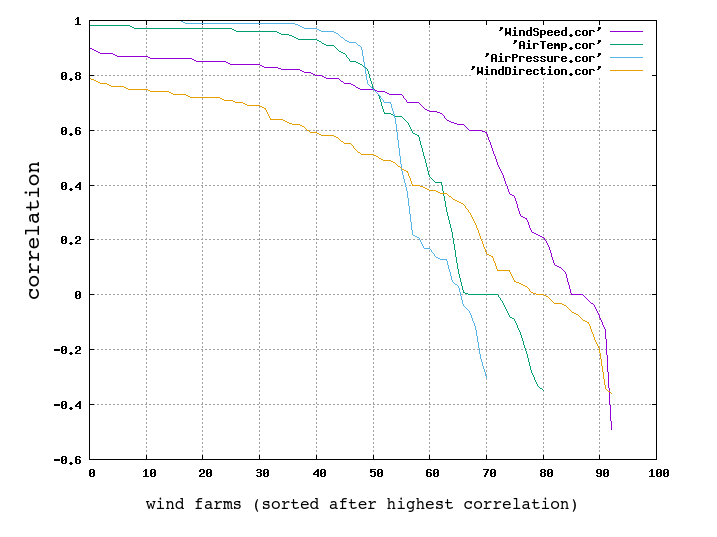
\includegraphics[width=0.75\textwidth]{figures/met_cor.png}
\caption{\textit{Results from a 2 year statistical verification of met data signals on CORRELATION for 4 variables. The x-axis shows wind farms ordered with the highest correlation first.}} 
\label{fig:met_cor}
\end{figure}


\begin{figure}[h!]
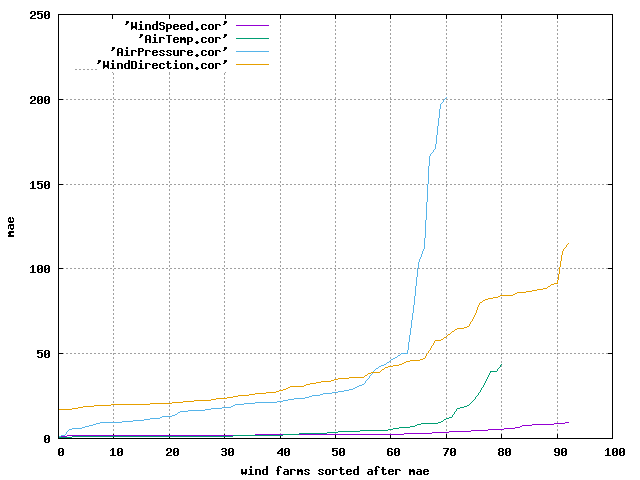
\includegraphics[width=0.7\textwidth]{figures/met_mae.png}
\caption{\textit{Results from a 2 year statistical verification of met data signals measured on MAE for 4 variables. The x-axis shows wind farms ordered with the lowest MAE first. The unit and magnitude is variable dependent and somewhat hides the growth of the wind speed error.}} 
\label{fig:met_mae}
\end{figure}


\begin{figure}[h!]
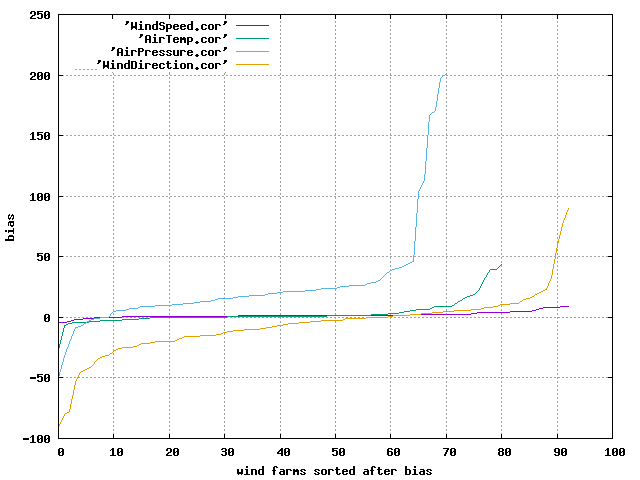
\includegraphics[width=0.7\textwidth]{figures/met_bias.png}
\caption{\textit{Results from a 2 year statistical verification of met data signals measured on BIAS for 4 variables. The x-axis shows wind farms ordered with the lowest BIAS first. The unit and magnitude is variable dependent. Note that the pressure BIAS hides the growth of the wind speed error for the last 30 wind farms.}} 
\label{fig:met_bias}
\end{figure}

With this graphical analysis it is possible to define acceptance limits for the quality of the data in terms of BIAS, MAE and CORRELATION.

\newpage

\subsection{QC for solar applications}

There are several sets of QC tests for historic radiation data (BSRN, SERI QC, QCRad, MESOR, ENDORSE, Journee et al., MDMS (Geuder et al.), ).
The tests in the literature use different limits for individual irradiance components (DHI, GHI, DNI) or parameters derived from these components together with solar position and at times clear sky irradiance. Types of limits are 
\begin{itemize}
    \item physical possible limits
    \item rare limits
    \item extremely rare limits
\end{itemize}
The existing QC tests have been harmonized in the framework of IEA PVPS Task 16 for stations with measurements of all three irradiance components (GHI, DHI, DNI) or two (GHI and DHI or DNI).
The quality control consists of automatic tests and visual inspection by an expert. The  QC results in one flag per time stamp and test. The flag's value is either "data seems ok", "data point was detected as problematic" or "test could not be performed". The latter can occur for a missing time stamp/data or if the test domain was not met and the test could not be applied.\\
The visual inspection of the data is of importance to detect bad data and manually assign the flag. This also includes the control of the meta data (logbook with comments, calibration information). Visual inspection can also help to determine if the time stamps refer to the end of the averaging interval (e.g. 1min, 10min or 1h averaging). The correct interpretation of the timestamps is essential. 
The following tests are defined. All test results are visualized and manual flagging can be used to improve the automatic test results. Some tests are not automated, but purely visual inspections:
\begin{itemize}
    \item   Missing time stamps	
    \item	Missing values	
    \item	K-Tests	
    \item	BSRN Three Component tests	
    \item	extremely rare limits test from BSRN	
    \item	Physically possible limits (PPL) test from BSRN
    \item	Tracker off test
    \item	Visual inspection: Heat map of irradiance with axes hour of the day (y) and day of year	 (x)
    \item	Visual inspection: Shading test: heat map of max irradiance in bins of Sun elevation and azimuth angle	with axes elevation (y) and azimuth (x)
    \item   Visual inspection: deviation of DNI measurement from DNI calculated from GHI and DHI	
    \item	Visual inspection: AM/PM symmetry of the time period	
    \item	Visual inspection: calibration changes by plot of the clear-sky index vs. time	
\end{itemize}



To decide if a data point can be used not only the result of a single flag per timestamp is needed, but all flags for that timestamp and surrounding timestamps must be considered. For the validation of satellite and model derived radiation data the following procedure is recommended. A data point is usable if all individual QC flags are indicating that the data is ok or that the test could not be performed and all measured radiation components are available. Also if 30 percent or more of the timestamps (daytime, solar elevation >0) from one day are flagged, exclude the entire day. Intervals between flagged data that are shorter than 60 min are also excluded. For the determination of the length of the interval only timestamps with elevation >0 are considered. Less stringent exclusion rules could be applied for other purposes, such as the determination of yearly sums.

\subsection{Historic QC other meteorological parameters {\color{red}{Comment from COM (21.08.2021: Do we really need that ? }}}

\section{Real time Quality Control (QC)}



%\subsection{Quality control in historic mode}\label{qa_historic} 
%{\color{green}{Comment from SW (28.06.2021: the text in the subsection "Quality control in historic mode" should be integrated in the subsections above}}
%% this text is now in section \label{subsubsec:qc_forecast_ranges}




%\subsubsection{Challenges and considerations for the QA process{\color{blue}{Author: COM -- needs more authors/discussion}}}\label{subsec:} 

\subsection{Real-time QC for Wind Applications}
{\color{blue}{Comment from COM (23.08.2021: Needs clean up!!! }}

\subsubsection{A. QC for Wind applications with Forecast Ranges}\label{subsubsec:real-time_qc_forecast_ranges}
One practical solution to test measurement signal quality is to use verification methods similar to the verification of forecast errors with the exception that a forecast or a forecast range is used as the reference, because it is the measurement that needs validation. The forecast has a known accuracy level, which is used to find changes in quality in the measurement signals....

\subsubsection{B. QC for Wind applications according to site assessement standards}\lebel{subsubsec:real-time_qc_site-assessment-standard}

For resource or site assessment in the planning phase of a wind farm an IEC standard exists \citep{iec17025-2005E} with an updated version 2 (IEC 61400-12-2:2013), that specifies which tests and what kind of criteria the instrumentation has to fulfil when used for the required tests to be carried out. The IEC 61400-12-2:2013 rules contain the following items:
\begin{itemize}
    \item Extreme winds
    \item Shear of vertical wind profile
    \item Flow inclination
    \item Background turbulence
    \item Wake turbulence
    \item Wind-speed distribution
\end{itemize}

The results of these tests have to be within a pre-defined range to be acceptable. In Appendix F of the 61400-12-1:2005 "Cup anemometer calibration procedure" the calibration of the instruments for measuring wind are specified \cite{iec61400-12-1-2005}.\\


MEASNET (MEASuring NETwork), the "international network for harmonised and recognized measurements in wind energy" has defined so called "Round Robin rules" for calibration of cup anemometers for wind energy \cite{measnet2009}, which are widely used. MEASNET has also  published a number of guidelines regarding instrument calibration and measurement campaigns for the wind industry within the EU project ACCUWIND (\cite{Dahlberg2006,Pedersen2006, Eecen2006}. Lee [2008] found a way of calibrating wind direction sensors with an optical camera.

The Annex D in IEC 61400-12-1:2005 standard states that the "implicit assumption of the method of this standard is that the 10 min mean power yield from a wind turbine is fully explained by the simultaneous 10 min mean wind speed measured at hub height, and the air density" [IEC, 2005, Annex D, Table D.1] and describes the associated measurement uncertainty evaluation principles.  In this respect, the standard refers to the "ISO Guide to the expression of Uncertainty in Measurements" \citep{jcgm2008,jcgm2009,jcgm2012} and its 2 supplements [\citep{jcgm2008a,jcgm2011} from the Joint Committee for Guides in Meteorology (JCGM), where there are two types of measurement uncertainty that are to be accounted for in any standardised measurement taking: 
\begin{enumerate}
    \item systematic errors, which are also known as measurement bias, often associated with offsets of the measured quantity
    \item random errors, which are associated with the fact that 2 measurements of the same quantity are seldom the same
\end{enumerate}

In section 3.1.2 of the guide, \citep{jcgm2008,jcgm2011} it is stated that "the result of a measurement .. is only an approximation or estimate .. of the value of the measurand and thus is complete only when accompanied by a statement of the uncertainty ... of that estimate". Considering this definition, all measurements should ideally have an uncertainty term associated with it. This is impractical in real-time operations, where the value of the measurements lies in the availability of the data at a given time. Therefore, it is unrealistic to request uncertainty measures. However, it could be a standing data value that is determined at the setup of the instrument and provided as part of the standing data. In that way, the instrument specific uncertainty could be accounted for in the handling of measurements.\\ 

The alternative is to carry out an uncertainty estimation with e.g. the Monte-Carlo method described in \citep{jcgm2011} pp23-33) or a mean uncertainty value must be added to raw measurements, as applied by Pinson and Hagedorn in an experiment over Ireland and Denmark with wind measurements from standard met masts [Pinson and Hagedorn, 2012 p7]. If a more standardised technical requirement is desirable, the JCGM guides offer a valuable general source, also applied in meteorology and oceanography. In that way, a harmonisation of "best practices" with these directly related real-time disciplines can be achieved. In fact, the guides do not only consider the measurand as a physical quantity, but also provide guidance to the conceptual design and the theoretical analysis of measurements and methods. 

In the introduction to the Guide [JCGM, 2009], it is stated that “..the principles of this Guide are intended to be applicable to a broad spectrum of measurements”, including those required for:
\begin{itemize}
   \item maintaining quality control and quality assurance in production
   \item complying with and enforcing laws and regulations
   \item calibrating standards and instruments and performing tests throughout a national 
   \item measurement system in order to achieve tractability to national standards developing, maintaining, and comparing international and national physical reference standards, including reference materials 
\end{itemize}

To summarise, the handling and integration of wind power into the electric grid is an equally important step to harness the full potential of the energy resource in an efficient and environmentally friendly way. 


This requires that measurements are trustworthy and maintained to a quality that allows for their use in forecasting tools in order to produce high quality forecasts and thereby reduce the need of reserves. These guides in combination with the IEC 61400-1 standard provide a good foundation for any grid code technical requirement specifications. 

In the following a few specific control procedures for the most common instrumentation are provided.  

\begin{enumerate}
    \item Cup anemometer on a met mast:\\

The accuracy of a single value from a cup anemometer is not high without a 10min time average. The purpose of the 10min averaging process is to eliminate the impact of the turbulent motion, which is generated as a result of frictional forces from the terrain on the air as well as the imbalance in the diurnal cycle and the temperature difference between the air and the surface.
From a 15 minute data delivery of a noise contaminated signal, it is almost impossible to prove the correctness or falsify the data  signals, because some of the values are realistic and others are not.

In contrast to the nacelle measurements, a single cup anemometer on a mast can be inspected at a much lower cost, today even with a drone. Several anemometers can be mounted on the mast and it is at least possible to submit the data directly without giving the wind farm software the possibility to delay, block or manipulate the data.

    \item Cup anemometer on a wind turbine nacelle:\\
      {\color{blue}{Author: COM -- needs more authors/discussion}}
    \item Remote sensing devices:\\
{\color{blue}{Author: COM -- needs more authors/discussion}}




    \item Blade-pressure computed nacelle wind:\\
{\color{blue}{Author: COM -- needs more authors/discussion -- there are areas, where this is used to a great extend and the results are astonishing good as a fit for the produced power. These methods are mainly used for wind farm control; nevertheless they have some important and interesting aspect also for real-time forecasting....}}


\end{enumerate}



\subsection{Real time  QC for solar Forecasting Applications}

For the real-time QC of solar radiation data, the QC methods for historic data can only be partly applied. QC methods requiring visual inspection cannot be applied automatically. Such methods can be used to analyse errors that are detected differently. QC results indicating that the result is suspicious such as the above described tests for rare limits or some versions of the three component tests might lead to too many data gaps, depending on the real-time application. If this is the case, these strict QCs should be adapted with less strict limits or used only for the further analysis of the data once another QC test was not passed. The limits should be defined based on the required data quality and data availability. A site dependence of these limits should be considered. For different instrument options different limits might be required, as e.g. cosine errors of pyranometers vary strongly between different models. Currently no standardised QC for real-time radiation data exist. 



\section{Real time QC other meteorological parameters {\color{red}{Comment from COM (21.07.2021: Do we really need that ? }}}






\chapter{Best Practice Recommendations {\color{magenta}{Contributing author: }}}
%\\ \color{green} POST PUBLIC REVIEW VERSION\color{black}}
\label{ch:bestpractice}

\noindent\begin{tcolorbox}
\parbox{\textwidth}{
\emph{\textbf{Key Points}\\
The recommendations in this section are based on the following set of principles:
\begin{itemize}
    \item 
    \item 
    \item 
    \item 
\end{itemize}
}}
\end{tcolorbox}

In this last chapter, the principles developed in the previous chapters are brought to the application level. In other words, the somewhat theoretical considerations from the previous chapters are now applied to real-world problems. 

%%%%%%%%%%%%%%%%%%%%%%%%%%%%%%%%%%%%%%%%%%%%%%%%%%%%%%%%%%%%%%%%%%%%%%%%%%%%%%%%%%%%%%%%%%%%%

\noindent\begin{tcolorbox}
\parbox{\textwidth}{
\emph{\textbf{Key Points}\\
Selection of instrumentation ...
}}
\end{tcolorbox}


\section{Instrumentation {\color{magenta}{Contributing author: }}}
 
    \subsection{Definitions }
 
    \subsection{Choice of instruments }
 
    \subsection{Verification of instrument signals }
    
     \subsubsection{Plausibility Analyses}\label{sec:plausibilityanalaysis}

\section{Requirements for the implementation into power grid operation {\color{magenta}{Contributing author: COM}}}
    
    \subsection{Implementation and Testing Rules }
    
    \subsection{Validation and Verification }
    
    \subsection{Maintenance Schedules }
    
\section{Requirements for the implementation into power plant operation {\color{magenta}{Contributing author: }}}
    \subsection{Implementation and Testing Rules }
    
    \subsection{Validation and Verification }
    
    \subsection{Maintenance Schedules }

\section{Quality Requirements {\color{magenta}{Contributing author: COM}} }\label{sec:data_quality_requirements}
    
    
    \subsection{Valid ranges }\label{subsec:validranges}
    
    
    \subsection{Valid error levels }\label{subsec:validerrors}




\newpage
%\printbibliography[heading=bibintoc]
%\label{bib/mybib}
%\input{bib/iearppart3.bib}
%\input{bib/biblio.tex}

%\printbibliography[heading=bibintoc]
%\section*{References}
%%\bibliographystyle{plain}
%\bibliography{bib/mybib}
%\begin{thebibliography}{27}
\chapter*{References}\label{references}
\setlength{\parindent}{-1cm}\\

%\bibitem{AESO2011a}
\noindent
%AESO, ISO rule 502-1: Wind Aggregated Generating Facilities Technical Requirements, 2011. Online:\small{\url{http://www.aeso.ca/downloads/502_1_Wind_Aggregated_Generating_Facilities_Technical_Requirements.pdf}} , \small{\url{http://www.aeso.ca/rulesprocedures/18592.html}} => Division 502-Technical Requirements.  

%\bibitem{AESO2011b}
AESO ISO rule 502-1: Wind Aggregated Generating Facilities Technical Requirements - Wind Forecasting Information. Online: \small{\url{http://www.aeso.ca/rulesprocedures/18592.html}} => Division 502 - 11-007R Wind Power Forecasting, \small{\url{http://www.aeso.ca/downloads/2011-06-23_Wind_Forecasting_ID.pdf}}

Allik, A. Uiga, J., Annuk, A.,  Deviations between wind speed data measured with nacelle-mounted anemometers on small wind turbines and anemometers mounted on measuring masts, Agronomy Research 12(2), 433­444, 2014.                      
Online: \small{\url{http://www.tuuleenergia.ee/wp-content/uploads/BSE-2014-renewable-energy\\-artikkel.pdf}}


Angelou, Nikolas et al. Doppler lidar mounted on a wind turbine nacelle – UPWIND deliverable D6.7.1 Roskilde: Danmarks Tekniske Universitet, Risø Nationallaboratoriet for Bæredygtig Energi. 2010. (Denmark. Forskningscentre Risoe. Risoe-R; Journal number 1757(EN)). 
Online: \small{\url{http://orbit.dtu.dk/en/publications/}}
%doppler-lidar-mounted-on-a-wind-turbine-nacelle--upwind-deliverable-d671(cde3bbcc-0663-4421-b75f-c976fdbc49a4).html"}


Ammonit Wind measurement. Online 2016-09-06:\\                          
\small{\url{http://www.ammonit.com/en/wind/wind-measurement}}


Ammonit, AQ 510 Classification Test, Online taken on 12.09.2016. Online: \small{\url{http://www.ammonit.com/en/news/news/521-aq510-classification-test}}


Antoniou I, Jørgensen HE, Mikkelsen T, Frandsen S, Barthelmie R, Perstrup C, Hurtig M. Offshore wind profile measurements from remote sensing instruments. In Proceedings of the European Wind Energy Association Conference and Exhibition. Athens, 2006.

Basu, S., Porté-Agel, F., Foufoula-Georgiou, E., Vinuesa, J-F. and Pahlow, M. (2006) Revisiting the Local Scaling Hypothesis in Stably Stratified Atmospheric Boundary-Layer Turbulence: an Integration of Field and Laboratory Measurements with Large-Eddy Simulations. Boundary-Layer Meteorology 18(3): 473-500.          
Online: \small{\url{http://dx.doi.org/10.1007/s10546-005-9036-2}}

Berg, L.K., M. Pekour, and D. Nelson: Description of the Columbia Basin Wind Energy Study (CBWES). Pacific Northwest National Laboratory Tech. Rep. PNNL-22036, 14 pp., 2012. Online: \small{\url{http://www.pnnl.gov/main/publications/external/technical_reports/PNNL-22036.pdf}}

Bing{\"o}l, F., Mann, J., Foussekis, D.: Conically scanning lidar error in complex terrain. Meteorologische Zeitschrift, 18 (2), pp. 189-195(7). Emeis, Stefan; Harris, Michael; Banta, Robert M., 2007: Boundary-layer anemometry by optical remote sensing for wind energy applications. Meteorologische Zeitschrift, 16 (4), pp. 337-347(11),2009a.

Bing{\"o}l, F., Complex Terrain and Wind Lidars. Ph.d. thesis, Risø DTU, 2009. Online: \small{\url{http://orbit.dtu.dk/fedora/objects/orbit:83301/datastreams/file_5245709/content}}

Blackadar, A. K., Boundary layer wind maxima and their significance for the growth of nocturnal inversions. Bull. Amer. Meteor. Soc., 38, 283-290, 1957. Online: \small{\url{http://twister.ou.edu/MM2005/Blackardar1957BAMS.pdf}}

BPA, Bonneville Power Adminstration's Technical Requirements for Interconnection to the BPA Transmission Grid, STD-N-000001, 2015. Online: \small{\url{https://www.bpa.gov/transmission/Doing\%20Business/Interconnection/Pages/default.aspx BPA_tech_requirements_interconnection.pdf}}

Bradley, S., Wind speed errors for LIDARs and SODARs in complex terrain; 14th International Symposium for the Ad

Bradley, S. Wind speed errors for lidars and sodars in complex terrain. IOP Conference Series: Earth and Environmental Science, 1(1):012061, 2008b. Online: \small{\url{http://stacks.iop.org/1755-1315/1/i=1/a=012061}}

Bradley, S., Y. Perrott, P. Behrens, and A. Oldroyd. Corrections for wind-speed errors from sodar and lidar in complex terrain. Boundary-Layer Meteorology, 143:37­48, 2012a. 
Online: \small{\url{http://dx.doi.org/10.1007/s10546-012-9702-0}}

Bradley, S., S. von Hünerbein, and T. Mikkelsen. A bistatic sodar for precision wind profiling in complex terrain. Journal of Atmospheric and Oceanic Technology, 29(8):1052­1061, 2012b. Online: \small{\url{http://dx.doi.org/10.1175/JTECH-D-11-00035.1}}

Burin des Roziers, E., REPEATABILITY OF ZEPHIR PERFORMANCE DEMONSTRATED ACROSS A SAMPLE OF MORE THAN 170 IEC COMPLIANT VERIFICATIONS, Report by ZephirLiDAR, 2014.  Online: \small{\url{http://www.ammonit.com/images/stories/download-pdfs/TestReports/Repeatability_of\\_ZephIR_performance.pdf}}

California ISO, Wind Technical Requirements, fifth Replacement California ISO Tariff archive, Appendix Q Eligible Intermittent Resources Protoco EIRP, 2014.   Online: \small{\url{http://www.caiso.com/rules//Pages/Regulatory/TariffArchive/Default.aspx}},\\ CALISO\_PIRP\_WindTechnicalRequirements02-Mar-2009.pdf,\\ AppendixQ\_EligibleIntermittentResourcesProtocolEIRP\_May1\_2014.pdf.


California ISO,  Business Practice Manual for Direct Telemetry, Version 9, p.57, May 2016. Online: \small{\url{http://www.caiso.com/rules/Pages/BusinessPracticeManuals/Default.aspx}}\\ -> Dokument: BPM\_for\_Direct\_Telemetry\_V9\_Clean.docx

Campbell, I., A Comparison of Remote Sensing Device Performance at Rotsea, Report by Renewable Energy Systems, Document Reference: 01485-000090 Issue: 05, 2011.
Online: \url{https://www.renewablenrgsystems.com/services-support/resources/documentation-and-downloads/white-papers/detail/a-comparison-of-remote-sensing-device-performance-at-rotsea}
	
Courtney, M., Wagner, R., Lindelöw, P., Commercial Lidar profilers for wind energy. A comparative guide. Proc. of European Wind Energy Conf., Brussels, 2008.
Online: \url{https://www.renewablenrgsystems.com/services-support/resources/documentation-and-downloads/white-papers/detail/commercial-\\lidar-profilers-for-wind-energy-a-comparative-guide},\\
\small\url{http://www.renewablenrgsystems.com/assets/resources/Commercial-Lidar-Profilers-for-Wind-Energy-Whitepaper.pdf}


Cuerva A., Sanz-Andrés A., Franchini S., Eecen P., Busche P., Pedersen T.F., Mouzakis F., "ACCUWIND ­ Accurate Wind Measurements in Wind Energy, Task 2. Improve the Accuracy of Sonic Anemometers, Final Report", UPM/IDR Madrid June 2006


Dahlberg J.-Å., Pedersen T.F., Busche P., "ACCUWIND ­ Methods for Classification of Cup Anemometers", Risø-R-1555(EN), May 2006.


Dahlberg, J-A., Frandsen, S. T., Aagaard Madsen, H., Antoniou, I., Friis Pedersen, T., Hunter, R., Klug, H., Is the nacelle mounted anemometer an acceptable option in performance testing? In E. L. Petersen, P. Hjuler 

Deutsche Windgard, Performance Verification of Galion, Report 13001, 2013. Online: \url{http://www.sgurrenergy.com/wp-content/uploads/2015/09/DWGGalion-Report.pdf}


DNVGL, Review of the Spinner anemometer from ROMO Wind iSpin, Report No.: 113605-DKAR-R-01, Rev. 3, Document No.: 113605-DKAR-R-01, 2015.           
Online: \small{\url{http://romowind.com/media/113605-DKAR-R-01\\ -Rev-3-2015-03-06.pdf}}


Drechsel, S., G. J. Mayr, J. W. Messner, R. Stauffer, Wind Speeds at Heights Crucial for Wind Energy: Measurements and Verification of Forecasts, J. Appl. Meteor. Climatol., 51, 1602-1617, 2012.


Eecen P.J., Mouzakis F., Cuerva, A "ACCUWIND, Work Package 3 Final Report", ECN-C-06-047, May 2006.


Emeis, S., Harris,M., Banta, R.M.,  Boundary-layer anemometry by optical remote sensing for Wind energy applications. Meteorologische Zeitschrift, 16(4):337{347, 2007.


Enevoldsen, K., Comparison of 3D turbulence measurements using three staring wind lidars and a sonic anemometer. IOP Conference Series: Earth and Environmental Science, 1(1):012012, 2008.
Online \small{\url{http://stacks.iop.org/1755-1315/1/i=1/a=012012}}


Environmental Protection Agency (EPA), Office of Air Quality, Planning and Standards, Meteorological Monitoring Guidance for Regulatory modelling Applications, Doc. EPA-454/R-99-005, 2000. Online:\small{\url{https://www3.epa.gov/scram001/guidance/met/mmgrma.pdf}}


ERCOT, ERCOT Business Practices: ERCOT AND QSE OPERATIONS PRACTICES DURING THE OPERATING HOUR, Version 5.5, April 2012.                              
Online:\url{http://www.ercot.com/mktrules/bpm} -> \\BP\_ERCOT\_And\_QSE\_Operations_Practices_v5_5.doc


EWEA, Wind Energy: The Facts Homepage, Best Practice for Accurate Wind Speed Measurements, Online extracted August 2016.                        
Online:\small{\url{http://www.wind-energy-the-facts.org/best-practice-for-accurate-\\wind-speed-measurements.html}}

\bibitem{EWELINE2011}
EWeLINE project: Development of innovative weather and power forecast models for the grid integration of weather dependent energy sources.      
Online: \small{\url{http://www.projekt-eweline.de/en/project.html}}


Falbe-Hansen, GL Garrad Hassan, Technology Review of the ROMO Wind Spinner Anemometer I, Document No. 111789-DKHI-R-01, 2012.
Online: \small{\url{http://romowind.com/media/GL-Garrad-Hassan-spinner-\\anemometer-report.pdf}}


Froese, M., Vattenfall and ROMO Wind publish performance data verifying accuracy of iSpin technology, Windenergy Enegineering&Development, Article from 25.May 2016. Online:\small{\url{http://www.windpowerengineering.com/featured/business-news-projects/vattenfall-romo\\-wind-publish-performance-data-\\verifying-accuracy-ispin-technology/2016_Froese_Windenergy-Eng-and-Dev_Romowind-\\Vattenfall-experiment-iSpin.pdf}}


G{\"o}{\cc}men T., Giebel G., Data-driven Wake Modelling for Reduced Uncertainties in short-term Possible Power Estimation: Paper. Journal of Physics: Conference Series, 1037(7), 072002, DOI:10.1088/1742-6596/1037/7/072002, 2018.


G{\"o}{\cc}men, T., Giebel, G., Estimation of turbulence intensity using rotor effective wind speed in Lillgrund and Horns Rev-I offshore wind farms, Renewable Energy, Vol. 99. pp. 524-532, 2016.


Grund, C.J.; Banta, R.M.; George, J.L.; Howell, J.N.; Post, M.J.; Richter, R.A.; Weickman, A.M., High-Resolution Doppler Lidar for Boundary Layer and Cloud Research, J.Atmospheric & Oceanic Technology (18), pp.376-393, 2001.


Hasager, Charlotte B.; Stein, Detlef; Courtney, Michael; Peña, Alfredo; Mikkelsen, Torben; Stickland, Matthew; Oldroyd, Andrew. 2013. "Hub Height Ocean Winds over the North Sea Observed by the NORSEWInD Lidar Array: Measuring Techniques, Quality Control and Data Management." Remote Sens. 5, no. 9: 4280-4303.


HECO, Hawaiian Electric Company, personal communication, October 2016.

IEA Wind Task 36: Wind Power Forecasting, 2016. Online: \url{http://www.ieawindforecasting.dk/}


IEA Wind Task 11: Best Technology Information Exchange Recommended Practices, Online: \small{\url{http://www.ieawind.org/task_11/recomend_pract.html}}


IEA Wind Task 11, Guideline 11  WIND SPEED MEASUREMENT AND USE OF CUP ANEMOMETRY, Second Edition, 2003.
Online: \small{\url{http://www.ieawind.org/task_11/recommended_pract/Recommended\\\%20Practice\%2011\%20Anemometry_secondPrint.pdf}}


IEA Wind Task 11, Guideline 15:  GROUND-BASED VERTICALLY-PROFILING REMOTE SENSING FOR WIND RESOURCE ASSESSMENT, First Edition, Jan. 2013.
Online: \small{\url{http://www.ieawind.org/task_11/recommended_pract/Recommended\%20Practice\%2015\%20RemoteSe\\nsing\%201stEd.pdf}}


IEC Standard 61400-12-1:2005(E)   “Wind   turbines   -   Part   12-1:   Power   perfor-mance measurements of electricity producing wind turbines, First edition 2005-12/ Annex F, “Cup anemometer calibration procedure”, 2005


IEC Standard 61400-12-1:2017, “Power performance measurements of electricity producing wind turbine”, 2017.


IEC/ISO 17025:2005(E), General requirements for the competence of testing and calibration laboratories, Version 2, 2005.
Joint Committee for Guides in Metrology, Evaluation of measurement data -- An introduction to the "Guide to the expression of uncertainty in measurement" and related documents, JCGM 104:2009, 2009.   
Online: \small{\url{https://en.wikipedia.org/wiki/Joint_Committee_for_Guides_in_Metrology}}

Jensen, K. Rave, P. Helm, & H. Ehmann (Eds.), Wind energy for the next millennium. Proceedings. (pp. 624-627). London: James and James Science Publishers, 1999.          
Online:\small{\url{https://www.etde.org/etdeweb/servlets/purl/679606/?type=download}}  (see pp.55ff).

Joint Committee for Guides in Metrology, Evaluation of measurement data -- Guide to the expression of uncertainty in measurement. JCGM 100:2008, 2008.


Joint Committee for Guides in Metrology, Evaluation of measurement data -- Supplement 1 to the "Guide to the expression of uncertainty in measurement" -- Propagation of distributions using a Monte Carlo method, JCGM 101:2008, 2008a.


Joint Committee for Guides in Metrology, Evaluation of measurement data -- Supplement 2 to the "Guide to the expression of uncertainty in measurement" -- Propagation of distributions using a Monte Carlo method, JCGM 102:2011, 2011.


Joint Committee for Guides in Metrology, Evaluation of measurement data -- The role of measurement uncertainty in conformity assessment, JCGM 106:2012, 2012.


Jones, L.E., Strategies and Decision Support Systems for Integrating Variable Energy Resources in Control centres for Reliable Grid Operations, Global Best Practices, Examples of Excellence and Lessons Learned, Report for the Department of energy under the Award Number DE-EE0001375, 2012.


Kelley, N.D., Jonkman, B.J., Scott G.N., Pichugina, Y.L., Comparing Pulsed Doppler LIDAR with SODAR and Direct Measurements for Wind Assessment, Proc. AWEA Wind Conference 2007, Ref. NREL/CP-500-41792, July, 2007. 
Online: \small{\url{http://www.nrel.gov/wind/pdf}s/41792.pdf}}


Kelly, N. D., M. Shirazi, D. Jager, S. Wilde, J. Adams, M. Buhl, P. Sullivan, and E. Patton, 2004: Lamar low-level jet program interim report. NREL/TP-500-34593. 
Online at \small{\url{http://www.nrel.gov/docs/fy04osti/34593.pdf}}


Kindler, D., Oldroyd, A., Macaskill, A., Finch, D., An eight month test campaign of the Qinetiq ZephIR system:  Preliminary results. Meteorol. Z.,  16(5):479-489, 2007.


Krishnamurthy, R., Choukulkar, A., Calhoun, R., Fine, J., Oliver, A. and Barr, K.S., Coherent Doppler lidar for wind farm characterization. Wind Energ., 16: 189-206. DOI: 10.1002/we.539, 2013.


Lang, S., McKeogh, E., LIDAR and SODAR Measurements of Wind Speed and Direction in Upland Terrain for Wind Energy Purposes, Remote Sens. 2011, 3, 1871-1901; doi:10.3390/rs3091871, 2011. Online: \url{http://www.mdpi.com/journal/remotesensing}


LitGRID, PERDAVIMOS SISTEMOS OPERATORIAUS TIPINĖS IŠANKSTINĖS PROJEKTAVIMO SĄLYGOS VĖJO ELEKTRINIŲ PARKO PRIJUNGIMUI PRIE 110 kV ĮTAMPOS ELEKTROS PERDAVIMO TINKLO, Nr. 47, 2010.
Online:\url{http://www.litgrid.eu/index.php/services/connection-to-the-\\transmission-grid-/585}


Lundquist, J., K. Lundquist, Eugene S. Takle, Matthieu Boquet, Branko Kosovi, Michael E., Rhodes1, Daniel Rajewski3, Russell Doorenbos, Samantha Irvin, Matthew L. Aitken1, Katja, Friedrich1, Paul T. Quelet1, Jiwan 
Rana1, Clara St. Martin1, Brian Vanderwende, 1Rochelle, Worsnop1, Lidar observations of interacting wind turbine wakes in an onshore wind farm, Renewable NRG Systems Whitepaper, Online September 2016. 
Online:\\\small{\url{https://www.renewablenrgsystems.com/services-support/resources/documentation-and-\\downloads/white-papers/detail/lidar-observations-of-interacting-wind-turbine-wakes\\-in-an-onshore-wind-farm}}

\bibitem{Marquis2012}
Marquis, M., Wilczak, J., Finley, C., Freedman, J., Wind Forecasting Improvement Project (WFIP) final report, National centre of Oceanographic and Atmospheric Administration (NOAA), 2014. 
Online: \url{http://energy.gov/sites/prod/files/2014/05/f15/wfipandnoaafinalreport.pdf} Project Homepage:  
\url{http://www.esrl.noaa.gov/psd/renewable_energy/wfip/}


Masson C, Smaili A, "Numerical Study of Turbulent Flow around a Wind Turbine Nacelle", Wind Energy, 9:281-298, 2006.


Matzler, C., Thermal Microwave Radiation: Applications for Remote Sensing, The Institution of Engineering and Technology, London, Chapter 1, 2006

MEASNET, Cup Anemometer Calibration Procedure – Version 2, October 2009.
Online: \url{http://www.measnet.com/wp-content/uploads/2011/06/measnet_anemometer_calibration_v2_oct_2009.pdf}


MEASNET, Evaluation of Site specific Wind conditions, Version 2, April 2016. 
Online:\url{http://www.measnet.com/wp-content/uploads/2016/05/Measnet_SiteAssessment_V2.0.pdf}


M{"\o}hrlen, C., J{\o}rgensen, J.U., A new algorithm for Upscaling and Short-term forecasting of wind power using Ensemble forecasts, Proc. of the 8th International Workshop on Large-Scale Integration of Wind Power into Power Systems as well as on Transmission Networks for Offshore Wind Farms, pp., 2009.                          
Online: \url{http://www.weprog.com/files/weprog_windintegration_2009_p54_paper.pdf}


M{\"o}hrlen, C., Uncertainty in Wind Energy Forecasting, PhD Thesis, pp19-21, 2004.
Online: \url{http://library.ucc.ie/record=b1501384~S0} full text: \url{http://hdl.handle.net/10468/193} 

Monserrat, S. and Thorpe, A. J. , Gravity-Wave Observations Using an Array of Microbarographs In the Alearic Islands. Q.J.R. Meteorol. Soc., 118: 259–282. doi:10.1002/qj.49711850405, 1992.


Morris, VR, Ceilometer Instrument Handbook, DOE/SC-ARM-TR-020, 2016.      Online: \url{http://www.arm.gov/publications/tech_reports/handbooks/ceil_handbook.pdf}

Morton, B., Osler, E., Coubart-Millet, G., Wind Iris Operational Applications, RNRG Whitepaper, 2016.
Online: \small{\url{https://www.renewablenrgsystems.com/services-support/resources/documentation-and-\\downloads/white-papers/detail/white-paper-wind-iris-operat\\ional-applications}}

NYISO, Wind Plant Operator Forecast Data Guide, June 2016. 	Online: \small{\url{http://www.nyiso.com/public/webdocs/markets_operations/documents/Manuals_and_Guides/Guides/User_Guides/Wind_Plant\\_Operator_Forecast_Data_Guide.pdf}}


Nakafuji, D., Making the elephant fly: Integrating distributed energy resources onto the grid in Hawaii, Guest Comment, published Online at Smart Electric Power Alliance webpage on 15.September 2016.
Online: \small{\url{http://www.solarelectricpower.org/utility-solar-blog/2016/september/making-the-elephant-\\fly-integrating-distributed-energy-resour\\ces-onto-the-grid-in-hawaii.aspx}}


Pedersen, T.F., Sørensen, N.,Enevoldsen, P., Aerodynamics and Characteristics of a Spinner Anemometer, Risø National Laboratory DTU Institute of Physics and IOP Publishing Limited, Doi: dx.doi.org/10.1088/1742-6596/75/1/012018, 2007. 
Online: \small{\url{http://www.risoe.dk/rispubl/art/2007_247.pdf}}


Pedersen, T.A., HA Madsen, R Møller, M Courtney, N Sørensen, Spinner anemometry - basic principles for application of the technology, 2016. 

Online: \small{\url{http://romowind.com/media/Spinner-anemometry-a-scientific-paper.pdf}}


Popinet, S., Murray Smith, and Craig Stevens, 2004: Experimental and Numerical Study of the Turbulence Characteristics of Airflow around a Research Vessel. J. Atmos. Oceanic Technol., 21, 1575–1589, doi: 10.1175/1520-0426(2004)021<1575:EANSOT> 2.0.CO;2.                                                                 

Pedersen T.F., Dahlberg J.-Å., Busche P., "ACCUWIND ­ Classification of Five Cup Anemometers According to IEC61400-12-1", Risø-R-1556(EN), May 2006.


Pedersen, F., Demurtas,T.G., Zahle, F., Calibration of a spinner anemometer for yaw misalignment measurements. Wind Energy, 18, 1933–1952. DOI: 10.1002/we.1798, 2015.
Online: \small{\url{http://orbit.dtu.dk/ws/files/99931702/Calibration_of_a_spinner_anemometer.pdf}}


Pe{\~n}a, A., Hasager, C. B., Lange, J., Anger, J., Badger, M., Bing{\"o}l, F.,.. Würth, I., Remote Sensing for Wind Energy. DTU Wind Energy.  (DTU Wind Energy E; No. 0029(EN)), 2013. Online: \small{\url{http://orbit.dtu.dk/files/55501125/Remote_Sensing_for_Wind_Energy.pdf}}


Pichugina, Yelena L., Robert M. Banta, W. Alan Brewer, Scott P. Sandberg, R. Michael Hardesty, Doppler Lidar-Based Wind-Profile Measurement System for Offshore Wind-Energy and Other Marine Boundary Layer Applications. J. Appl. Meteor. Climatol., 51, 327-349.DOI: 10.1175/JAMC-D-11-040.1, 2012.


Pichugina, Yelena L., Sara C. Tucker, Robert M. Banta, W. Alan Brewer, Neil D. Kelley, Bonnie J. Jonkman, Rob K. Newsom, 2008: Horizontal-Velocity and Variance Measurements in the Stable Boundary Layer Using Doppler Lidar: Sensitivity to Averaging Procedures. J. Atmos. Oceanic Technol., 25, 1307-1327. DOI: 10.1175/2008JTECHA988.1, 2008.


Pinson, P., and R. Hagedorn, Verification of the ECMWF ensemble forecasts of wind speed against observations. Meteor. Appl.,1-20, doi:10.1002/met.283, 2012. Online:\\\small{\url{http://www.ecmwf.int/en/elibrary/11679-verification-ecmwf-ensemble-forecasts-\\wind-speed-against-observations}}


PJM, Generator Operational Requirements, Manual 14D, Rev. 38, Effective Date: June 1, 2016. 	Online:\small{\url{http://www.pjm.com/documents/manuals.aspx}}


ROMOWIND, Knowledge Base: Free Data Access to the Noerrekaer Windfarm, Online (2016-09-05): Online: \url{http://www.romowind.com/en/open-dataScintec}, Datasheet Sodar wind profiler MFAS, Version 2012. 
Online: \url{http://www.scintec.com/english/Web/scintec/Details/A032002.aspx}


Scipi{\'o}n, D., Palmer, R., Chilson, P., Fedorovich, E., Botnick, A., Retrieval of convective boundary layer wind field statistics from radar profiler measurements in conjunction with large eddy simulation, Meteorologische Zeitschrift, Volume 18, Number 2,  pp. 175-187(13), 2009. 


Sj{\"o}holm,M., Mikkelsen, T., Mann, J., Enevoldsen, I and Courtney, M.,Time series analysis of continuous-wave coherent Doppler Lidar wind measurements. IOP Conf. Ser.: Earth Environ. Sci., 1, 012051. DOI: 10.1088/1755-1315/1/1/012051, 2008.


Smith DA, Harris M, Coffey AS, Mikkelsen T, Jørgensen HE, Mann J, Danielian R. Wind lidar evaluation at the Danish wind test site in Høvsøre. Wind Energy 2006; 9:87-93.


Smith, B., Link, H., Randall, G., McCoy, T., Applicability of Nacelle Anemometer Measurements for Use in Turbine Power Performance Tests, Proc. American Wind Energy Association Windpower Conference, NREL Report NREL/CP-500-32494, 2002. Online: \url{http://www.nrel.gov/docs/fy02osti/32494.pdf}


Tordoff, S., How to plan the perfect wind measurement campaign, Wind Power Monthly Online, March, 1, 2013. Online: \url{http://www.windpowermonthly.com/article/1172038/plan-\\perfect-wind-measurement-campaign}


Ulaby, F.T.,Moore,R.K. Fung. A.K., Microwave Remote Sensing—Active and Passive”. By F. T. Ulaby. R. K. Moore and A. K. Fung. (Reading, Massachusetts: Addison-Wesley,  Volume I: Microwave Remote Sensing Fundamentals and Radiometry, 1981.


Wagner, R., and Davoust, S., Nacelle lidar for power curve measurement  - Avedøre campaign. DTU Wind Energy.  (DTU Wind Energy E; No. 0016), 2013. Online: \url{http://orbit.dtu.dk/ws/files/53801282/Aved_re_campaign.pdf}


Wagner, R., Bejdic, J., Windcube + FCR test in Hrgud, Bosnia \& Herzegovina, DTU Wind Energy Report E-0039, March 2014. Online: \small{\url{http://orbit.dtu.dk/en/publications/windcube--fcr-test-at-hrgud\\-bosnia-and-herzegovina(de4febab-3ce2-435c-9aba-\\0583d677981c).html}}


Warmbier,G., Albers, F., Hanswillemenke, K., Verification of wind energy related measurements with a SODAR system, Proc. AWEA Windpower Conference, Pitsburg, 2006.
Online: \small{\url{https://www.environmental-expert.com/articles/verification-of-wind-energy-re\\lated-measurements-with-a-sodar-system-393158}}


Wikipedia, Sigma Coordinate System, Online:                          \small{\url{https://en.wikipedia.org/wiki/Sigma_coordinate_system}}


Wilczak, J. M., and Coauthors, 1995: Contamination of wind profiler data by migrating birds: Characteristics of corrupted data and potential solutions. J. Atmos.  Oceanic Technol., 12, 449­467, doi:10.1175/1520-0426(1995)012<0449:COWPDB>2.0.CO;2., 1995.


Wilczak, J. M., E. E. Gossard, W. D. Neff, and W. L. Eberhard, Ground-based remote sensing of the atmospheric boundary layer: 25 years of progress, Boundary-Layer Meteorol., 78, 321-349, 1996.


Wilczak,J.,Cathy Finley, Jeff Freedman, Joel Cline, Laura Bianco, Joseph Olson, Irina Djalalova, Lindsay Sheridan, Mark Ahlstrom, John Manobianco, John Zack, Jacob R. Carley, Stan Benjamin, Richard Coulter, Larry K. Berg, Jeffrey Mirocha, Kirk Clawson, Edward Natenberg, and Melinda Marquis,  The Wind Forecast Improvement Project (WFIP): A Public–Private Partnership Addressing Wind Energy Forecast Needs. Bull. Amer. Meteor. Soc., 96, 1699–1718, doi: 10.1175/BAMS-D-14-00107.1.,2015. Online: \small{\url{http://journals.ametsoc.org/doi/abs/10.1175/BAMS-D-14-00107.1}}
Wikipedia "Remote Sensing", Online on 5th September 2016: \small{\url{https://en.wikipedia.org/wiki/Remote_sensing}}


W{\"u}rth, I., and Valldecabres, L. and Simon, E. and M{\"o}hrlen, C. and Uzunoglu, B. and Gilbert, C. and Giebel, G. and Schlipf, D. and Kaifel, A., Minute-Scale Forecasting of Wind Power - Results from the collaborative workshop of IEA Wind Task 32 and 36, Energies 2019, 12, 712. Online \url{https://www.mdpi.com/1996-1073/12/4/712}.


Yang, Q., Berg, L.K.,, Pekour, M., Fast, J.D., Newsom, R.K., Evaluation of WRF-Predicted Near-Hub-Height Winds and Ramp Events over a Pacific Northwest Site with Complex Terrain, J. of Appl. Meteo. and Climatology, Vol. 52, p1753-1763, DOI: 10.1175/JAMC-D-12-0267.1, 2013.


Zhong, S., J. D. Fast, and X. Bian, A Case Study of the Great Plains Low-Level Jet Using Wind Profiler Network Data and a High - Resolution Mesoscale Model.  Mon. Wea. Rev.  , 124, pp785–806, 1996.
Online: \small{\url{http://journals.ametsoc.org/doi/abs/10.1175/1520-493(1996)124\%3C0785\%3AACSOTG\%3E2.0.CO\%3B2}}


Zahle, F., & Sørensen, N. N. (2009). Characterisation of the unsteady flow in the nacelle region of a modern wind turbine. In Proc. of the European Wind Energy Conference, 2009.
Online:  
\small{\url{http://orbit.dtu.dk/en/publications/characterization-of-the-unsteady-flow-in-\\the-nacelle-r}egion-of-a-modern-wind-turbine(392515e0-e420-4e3e-a0a7-4979700c5a19)/\\export.html}

\setlength{\parindent}{0in}
%\end{thebibliography}
%\bibliography{bib/references}

\appendix
\chapter{Examples of System Operator Met Measurement Requirements}\label{ch:requiremenexamples}

%collection of a few examples and reference or establish a table that compares some of the requirements of some of the major system operators in North America and Europe (and maybe elsewhere if we can find the info)?

\section{Comparison of Requirements in various jurisdictions}

\begin{itemize}
    \item \textbf{AESO}: Alberta Electric System Operator in Calgary, Alberta, Canada [AESO,2011]
    \item \textbf{CAISO}: California Independent System Operator [CAISO, 2014, 2016]
    \item \textbf{BPA}: Bonneville Power Administration in Portland, Oregon, USA [BPA, 2015]
    \item \textbf{ERCOT}: Electricity Council of Texas in Austin, Texas, USA [ERCOT, 2012]
    \item \textbf{NYISO}: New York Independent System Operator in Rensselaer,NY,USA [NYISO, 2016] 
    \item \textbf{PJM}: Independent System Operator in Audubon, PA, USA [PJM, 2016]
    \item \textbf{HECO}: Hawaiian Electric Company, Maoui, Hawaii [HECO, 2016]
    \item \textbf{LitGrid}: in Vilnius, Lithuania [LiTGRID, 2010]
\end{itemize}


\section{Met Measurement Example from Califorina Independent System Operator in USA}

\section{Met Measurement Example from Alberta Electric System Operator in Canada}

\section{Met Measurement Example from Irish System Operator EIRGRID Group}


\chapter{Statistical Metrics}\label{appB:metrics}

\begin{figure}[h!]
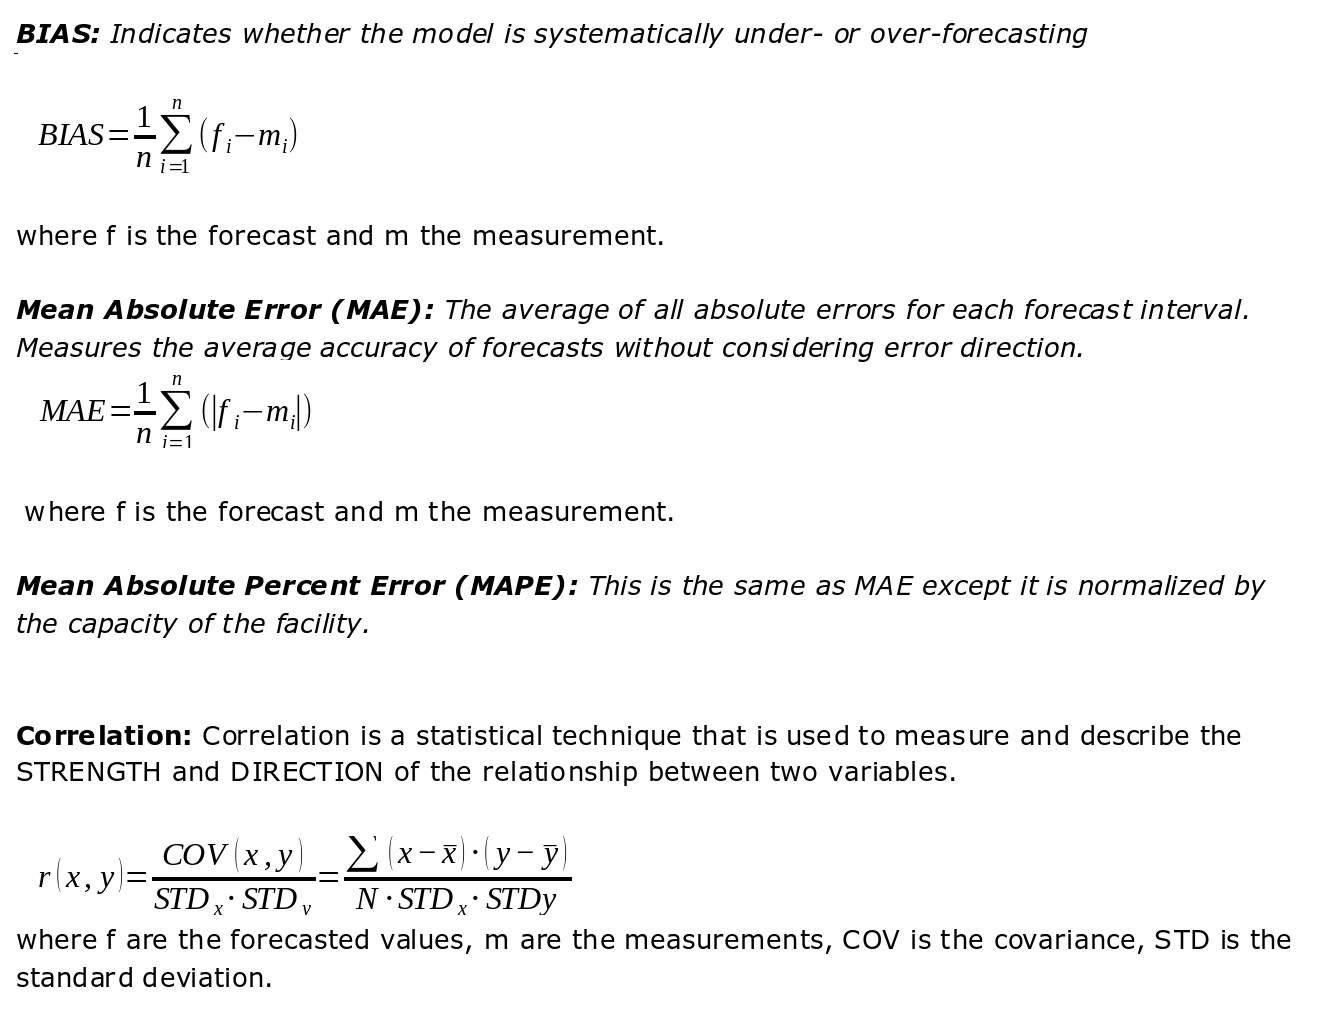
\includegraphics[width=0.9\textwidth]{figures/metrics.png}
\label{fig:figure2}
\end{figure}

\end{document}